% !TEX root = saveliev_physics_general_course_2.tex
%!TEX TS-program = pdflatex
%!TEX encoding = UTF-8 Unicode


\chapter{ĐIỆN TRƯỜNG TRONG CHÂN KHÔNG}\label{chap:1}

\section{Điện Tích}\label{sec:1_1}

Tất cả các vật thể trong tự nhiên đều có thể bị nhiễm điện, hay nhận điện tích. Khi vật thể bị nhiễm điện, nó sẽ tương tác với một vật thể nhiễm điện khác. Có hai loại điện tích tồn tại. Nó thường được gọi là điện tích dương và âm. Những điện tích cùng dấu thì hút nhau, trái dấu thì đẩy nhau.

Điện tích là một phần tử được cấu thành từ các hạt nguyên tố\footnote{Hạt nguyên tố được định nghĩa là những hạt vi mô mà với trình độ vật lý hiện tại, nội cấu trúc của nó không được coi như được cấu tạo từ những hạt khác.}. Điện tích của tất cả các hạt nguyên tố (trừ khi nó không tồn tại) có độ lớn như nhau. Nó được gọi là \textbf{điện tích nguyên tố}. Chúng ta sẽ sử dụng biểu tượng $e$ để ký hiệu cho điện tích nguyên tố dương. 

Những hạt nguyên tố bao gồm electron (mang điện tích âm), proton (mang điện tích dương), và neutron (không mang điện tích). Những hạt này là nền tảng để tạo nên nguyên tử, phân tử của tất cả vật thể, và vì thế tất cả vật thể đều có điện tích. Trong các vật thể, những hạt có dấu trái nhau có số lượng bằng nhau và phân bố với mật độ như nhau. Tổng đại số của tất cả các điện tích trong trường hợp này thì bằng không, và mỗi thể tích nguyên tố (cũng như là trên toàn bộ vật thể) sẽ trung hoà về điện tích. Nếu bằng một cách nào đó chúng ta tăng thêm số lượng hạt cùng dấu trong vật thể (cũng như là giảm bớt số lượng hạt ngược dấu), thì vật thể sẽ bị tích điện. Hơn nữa, hoàn toàn khả thi để tích điện mà không cần thay đổi tổng số lượng hạt âm và dương, chỉ cần phân bố lại điện tích trong vật thể. Việc này khiến cho một phần của vật thể có thừa điện tích của một dấu và phần khác bị thừa điện tích ngược dấu. Điều này có thể được thực hiện bằng việc đưa một vật thể tích điện đến gần kim loại chưa tích điện.

Vì điện tích $q$ được tạo nên bởi một số nguyên các $e$, nên
\begin{equation}\label{eq:1_1}
	q = \pm N e.
\end{equation}

\noindent
Một điện tích cơ bản rất nhỏ, đến nỗi các vật mang điện tích vĩ mô có thể được coi là mang điện tích phân bố liên tục.

Nếu một đại lượng vật lý chỉ có thể nhận các giá trị rời rạc, thì nó được gọi là bị lượng tử hoá. Điều này đã được chỉ ra trong \eqn{1_1}, rằng điện tích bị lượng tử hoá. 

Độ lớn của một điện tích là như nhau trong mọi hệ quy chiếu quán tính. Vì thế, điện tích được cho là có tính chất bất biến tương đối tính. Điều này dẫn đến việc độ lớn của điện tích không phụ thuộc vào trạng thái của điện tích là đứng yên hay di chuyển.

Điện tích có thể biến mất và xuất hiện lại. Hai điện tích cơ bản khác dấu tồn tại và biến mất tại cùng một thời điểm. Ví dụ, một electron và một positron (positron là electron mang điện tích dương) khi tiếp xúc với nhau sẽ xảy ra hiện tượng sự hủy hạt, khi đó chúng biến thành một gamma-photon trung hoà về điện. Điều này xảy ra là bởi sự biến mất của $-e$ và $+e$. Ngược lại, trong quá trình sinh cặp, một gamma-photon đi vào trường của một hạt nhân nguyên tử, và biến thành một cặp hạt---một electron và một positron. Quá trình này sinh ra điện tích $-e$và $+e$.

Như vậy, tổng điện tích của hệ mang điện cô lập\footnote{Một hệ mang điện được coi là cô lập nếu như không một bất cứ điện tích nào có thể thoát khỏi hoặc thêm vào hệ thông qua biên giới của hệ} là không đổi. Đây chính là phát biểu của \textbf{định luật bảo toàn điện tích}.

Chúng ta cần lưu ý rằng, định luật bảo toàn điện tích liên hệ mật thiết với sự bất biến tương đối tính của điện tích. Vì nếu độ lớn của điện tích phụ thuộc vào vận tốc của nó, vậy thì khi ta dời một điện tích của một dấu, chúng ta sẽ kiến tổng điện tích của hệ cô lập bị thay đổi.

\section{Định luật Coulomb}\label{sec:1_2}

Định luật được tuân theo bởi lực tương tác của các điện tích điểm được thực nghiệm thành lập vào năm 1785 bởi nhà vật lý người Pháp Charles A. de Coulomb (1736-1806). Một \textbf{điện tích điểm} được định nghĩa là một vật mang điện mà kích thước của nó có thể bỏ qua khi so với khoảng cách từ nó tới những vật thể mang điện khác.

Sử dụng một cái cân xoắn (\fig{1_1}) tương tự với cái được sử dụng bởi H. Cavendish để xác định hằng số hấp dẫn (xem Vol. I, Sec. 6.1), Coulomb đo được lực tương tác của hai quả cầu mang điện phụ thuộc vào độ lớn điện tích của chúng và khoảng cách giữa chúng. Ông ấy bắt đầu từ thực tế rằng khi một quả cầu kim loại mang điện tiếp xúc với một quả cầu giống hệt nhưng không mang điện, điện tích sẽ được phân bố như nhau giữa hai quả cầu.

\begin{figure}[!htb]
	\begin{center}
		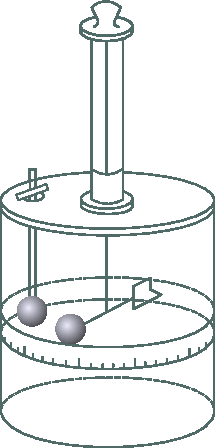
\includegraphics[scale=0.9]{figures/ch_01/fig_1_1.pdf}
		\caption[]{}
		\label{fig:1_1}
	\end{center}
	\vspace{-0.8cm}
\end{figure}

Như là kết quả từ thực nghiệm, Coulomb dẫn đến kết luận rằng \textit{lực tương tác giữa hai điện tích điểm đứng yên tỷ lệ thuận với độ lớn điện tích của mỗi hạt và tỷ lệ nghịch với bình phương khoảng cách giữa chúng}. Hướng của lực trùng với đường thẳng nối các điện tích.

Cần lưu ý rằng hướng của lực tương tác dọc theo đường thẳng nối các điện tích điểm đến từ việc xem xét tính đối xứng. Một không gian trống được giả định là đồng tính và đẳng hướng. Kết quả là, hướng duy nhất khác biệt trong không gian chứa các điện tích tĩnh là từ một điện tích tới các điện tích khác. Giả sử rằng lực $\vec{F}$ tác dụng lên điện tích $q_i$ (\fig{1_2}) tạo một góc $\alpha$ với hướng từ $q_1$ tới $q_2$, và $\alpha$ khác $0$ hoặc $\pi$. Nhưng do tính đối xứng trục, không có căn cứ để xác định lực  $\vec{F}$ khỏi vô số các lực có hướng khác nhưng đều tạo góc  $\alpha$ với trục $q_1$-$q_2$ (hướng của các lực này tạo thành một hình nón với góc ở đỉnh $2\alpha$). Khó khăn xuất hiện như kết quả của điều này biến mất khi $\alpha$ bằng $0$ hoặc $\pi$.

\begin{figure}[!htb]
	\begin{minipage}[t]{0.5\linewidth}
		\begin{center}
			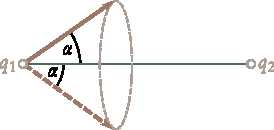
\includegraphics[scale=1]{figures/ch_01/fig_1_2.pdf}
			\caption[]{}
			\label{fig:1_2}
		\end{center}
	\end{minipage}
	\hspace{-0.05cm}
	\begin{minipage}[t]{0.5\linewidth}
		\begin{center}
			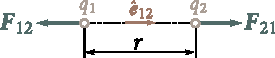
\includegraphics[scale=1]{figures/ch_01/fig_1_3.pdf}
			\caption[]{}
			\label{fig:1_3}
		\end{center}
	\end{minipage}
\vspace{-0.4cm}
\end{figure}

Định luật Coulomb có thể được biểu diễn thông qua biểu thức
\begin{equation}\label{eq:1_2}
	\vec{F}_{12} = -k \frac{q_1 q_2}{r^2}\,\vecuni{12}.
\end{equation}

\noindent
Ở đây, $k$ là một hằng số tỷ lệ được cho là dương, $q_1$ và $q_2$ là độ lớn của những điện tích tương tác, $r$ là khoảng cách giữa các điện tích, $\vecuni{12}$ là vector đơn vị hướng từ điện tích $q_1$ tới $q_2$ và $\vec{F}_{12}$ là lực tác dụng lên điện tích $q_1$ (\fig{1_3}; hình ảnh tương ứng cho trường hợp này).

Lực $\vec{F}_{21}$ khác $\vec{F}_{12}$ ở dấu của nó:
\begin{equation}\label{eq:1_3}
	\vec{F}_{21} = k \frac{q_1 q_2}{r^2}\,\vecuni{12}.
\end{equation}

Độ lớn của lực tương tác, là như nhau cho cả hai điện tích, có thể được viết ở dạng
\begin{equation}\label{eq:1_4}
	F = k \frac{\absolute{q_1 q_2}}{r^2}.
\end{equation}

Thí nghiệm chỉ ra rằng lực tương tác giữa hai điện tích đã cho không đổi khi có các điện tích khác đặt gần chúng. Giả sử chúng ta có điện tích $\ab{q}{a}$ và, thêm vào đó, $N$ điện tích khác $q_1, q_2,\ldots, q_N$. Từ trên có thể thấy rằng lực tổng hợp $\vec{F}$ từ $N$ điện tích $q_i$ tác dụng lên $\ab{q}{a}$ là
\begin{equation}\label{eq:1_5}
	\vec{F} = \sum_{i=1}^N \ab{\vec{F}}{a, $i$}
\end{equation}

\noindent
Với $\ab{\vec{F}}{a, $i$}$ là lực mà điện tích $q_i$ tác dụng lên $\ab{q}{a}$ trong sự có mặt của $N-1$ điện tích khác.

Thực tế thể hiện bởi \eqn{1_5} cho phép chúng ta tính toán lực tương tác giữa những điện tích tập trung trên các vật thể có kích thước hữu hạn, nhờ định luật của sự tương tác giữa các điện tích điểm. Với mục đích này, chúng ta phải chia mỗi vật mang điện thành những điện tích nhỏ $\deriv{q}$ có thể coi như chất điểm, sử dụng \eqn{1_2} để tính lực tương tác giữa các cặp điện tích $\deriv{q}$, sau đó thực hiện tổng hợp vector từ những lực này. Về mặt toán học, phương pháp này hoàn toàn giống với việc tính toán lực hấp dẫn giữa các vật thể có kích thước hữu hạn (xem Vol. I, Sec. 6.1).

Tất cả dữ kiện thực nghiệm có sẵn dẫn đến kết luận rằng định luật Coulomb sử dụng được cho khoảng cách từ \SI{e-15}{\metre} tới ít nhất vài kilomet. Có cơ sở để cho rằng định luật không còn đúng nữa đối với khoảng cách nhỏ hơn \SI{e-16}{\metre}. Với khoảng cách rất lớn, Không có sự xác nhận thực nghiệm cho định luật Coulomb. Nhưng cũng không có lý do để cho rằng định luật này không còn được tuân thủ với khoảng cách rất lớn giữa các điện tích.

\section{Hệ Thống Đơn Vị}\label{sec:1_3}

Chúng ta có thể tạo một hằng số tỉ lệ trong phương trình \eqn{1_2} bằng cách chọn đơn vị cho điện tích (đơn vị của $F$ và $r$ đã được thành lập trong cơ học). Đơn vị của điện tích (khi $F$ và $r$ được đo trong hệ đơn vị cgs) được gọi là \textbf{đơn vị tĩnh điện tuyệt đối} của điện tích (cgse$_q$). Nó là độ lớn của hai điện tích giống nhau tương tác với nhau qua một lực \SI{1}{\dyne} và cách nhau chúng cách nhau \SI{1}{\centi\metre}

Đo lường chi tiết (được mô tả ở \sect{10_3}) cho ta biết giá trị điện tích cơ bản là
\begin{equation}\label{eq:1_6}
	e = \num{4.80e-10}\text{cgse$_q$}.
\end{equation}

Giống như các đơn vị cơ bản như độ dài, khối lượng, thời gian, thì điện tích cũng là một đơn vị cơ bản mà chúng ta dùng để xây dựng hệ thống đơn vị của điện từ học. Hệ thống dựa trên các đơn vị như centimet, gram, giây, và cgse$_q$ còn được gọi là \textbf{hệ thống đơn vị tĩnh điện tuyệt đối} (hệ thống cgse). Nó được tìm ra bởi định luật Coulomb, hay định luật tương tác giữa các điện tích nghỉ. Trong những phần sau, chúng ta sẽ trở nên quen thuộc với \textbf{hệ thống đơn vị điện từ tuyệt đối} (hệ thống cgsm), hệ thống này dựa trên các định luật tương tác giữa các vật dẫn mang dòng điện. Hệ Gauss cũng sử dụng các đơn vị giống với cả hệ thống cgse và cgsm, và nó cũng là một hệ thống đơn vị tuyệt đối.

Phương trình \eqref{eq:1_4} trong hệ cgse sẽ trở thành
\begin{equation}\label{eq:1_7}
	F = \frac{\absolute{q_1 q_2}}{r^2}.
\end{equation}

\noindent
Phương trình chỉ đúng đối với môi trường đang xét là chân không. Nó cần phải xem xét kĩ hơn nếu xét trong môi trường là điện môi.

USSR State Standard GOST 9867-61 có hiệu lực vào ngày 1, tháng 1, 1963, đề xuất về việc sử dụng Hệ Thống Đơn Vị Quốc Tế (SI). Những đơn vị cơ bản trong hệ thống này là mét, kilogram, giây, ampere, kelvin, candela, và mole. Đơn vị của lực trong hệ SI là (\si{\newton}) bằng với \num{e5} dynes. 

Để thành lập các đơn vị trong hệ SI cho các đại lượng điện từ học, ta có thể suy ra từ các định luật. Giống như trong hệ cgsm, các đơn vị được suy ra từ định luật tương tác giữa các vật mang dòng điện. Điều đó dẫn đến việc, hằng số tỉ lệ trong phương trình Coulomb sẽ là đại lượng có thứ nguyên và riêng biệt so với các đơn vị khác.

Đơn vị SI của điện tích là Coulomb (\si{\coulomb}. Nó đã được tìm ra bởi các đo đạc thực nghiệm
\begin{equation}\label{eq:1_8}
	\SI{1}{\coulomb} = \num{2.998e9} \approx \num{3e9}{\text{ cgse$_q$}}.
\end{equation}

Để tìm giá trị của một đơn vị điện tích, ta sẽ đi tính toán lực tương tác giữa hai điện tích có giá trị \SI{1}{\coulomb} và chúng cách nhau \SI{1}{\metre}.
\begin{equation}\label{eq:1_9}
	F = \frac{\num{3e9}\times\num{3e9}}{100^2}\,\text{ cgse$_F$} = \SI{9e14}{\dyne} = \SI{9e9}{\newton} \approx \SI{e9}{\kgf}.
\end{equation}

Một điện tích cơ bản có thể được biểu diễn trong coulombs là
\begin{equation}\label{eq:1_10}
	e = \SI{1.60e-19}{\coulomb}.
\end{equation}

\section{Hiệu Chỉnh Các Công Thức}\label{sec:1_4}

Có nhiều công thức trong điện từ học khi được viết trong hệ cgs (đặc biệt trong hệ Gauss) có thành phần $4\pi$ và hằng số tốc độ ánh sáng trong chân không $c$. Để loại bỏ những thành phần này ra khỏi công thức, mà quan trọng trong thực tiễn, ta cho hằng số tỉ lệ trong định luật Coulomb bằng $1/4\pi\varepsilon_0$. Phương trình của điện tích trong chân không trở thành
\begin{equation}\label{eq:1_11}
	F = \frac{1}{4\pi\varepsilon_0}\frac{\absolute{q_1 q_2}}{r^2}.
\end{equation}

\noindent
Những công thức khác cũng thay theo đó. Việc thay đổi cách viết công thức được gọi là \textbf{hiệu chỉnh}. Hệ thống đơn vị được cấu tạo từ những công thức được hiệu chỉnh cũng được gọi là \text{hiệu chỉnh}.

Đại lượng $\varepsilon_0$ được gọi là \textbf{hằng số điện}. Nó có thứ nguyên là điện dung trên độ dài. Nó còn được biểu diễn dưới đơn vị farad trên mét. Để tìm được giá trị của $\varepsilon_0$, chúng ta sẽ tìm giá trị của lực tương tác trong \eqn{1_11} giữa hai điện tích có giá trị \SI{1}{\coulomb}, và chúng cách nhau \SI{1}{\metre}. Theo \eqn{1_9}, lực tương tác trong trường hợp này là \SI{9e9}{\newton}. Sử dụng giá trị này của lực, cũng như $q_1=q_2=\SI{1}{\coulomb}$ và $r=\SI{1}{\metre}$ vào phương trình \eqn{1_11}, chúng ta sẽ có được
\begin{equation*}
	\num{9e9} = \frac{1}{4\pi\varepsilon_0}\frac{\absolute{1\times 1}}{1^2}
\end{equation*}

\noindent
Hay
\begin{equation}\label{eq:1_12}
	\varepsilon_0 = \frac{1}{4\pi\times\num{9e9}} = \SI{0.885e-11}{\faraday\per\metre}.
\end{equation}

Hệ thống đơn vị Gauss được sử dụng rộng rãi, và tiếp tục được sử dụng trong công đồng vật lý. Vì thế, chúng ta xem trọng việc giúp các độc giả làm quen với cả hệ SI và hệ Gauss. Chúng ta nên trình bày các đại lượng trong đơn vị SI và Gauss cùng một lúc trong cùng một công thức. Các công thức quan trọng trong điện từ học trong cả hệ SI và Gauss được so sánh trong \app{A_3}

\section{Điện Trường.Cường Độ Điện Trường}\label{sec:1_5}

Một điện tích nghỉ tương tác thông qua một trường điện\footnote{Chúng ta sẽ thấy trong \sect{6_2}, nếu một điện tích đang di chuyển, nó còn tạo ra từ trường.}. Một điện tích làm thay đổi tính chất của môi trường xung quanh nó---nó sẽ tạo ra một trường điện. Nếu đặt một điện tích trong trường, nó sẽ chịu một lực. Vì thế, để tìm xem có điện trường không, ta chỉ cần đặt một vật thể nhiễm điện (từ giờ, chúng ta sẽ gọi ngắn gọn là điện tích) trong trường và xem xét lực tác dụng lên điện tích đó.

Do đó, để tìm hiểu và nghiên cứu về điện trường, chúng ta sẽ sử dụng đến điện tích ``thử''. Để lực tác dụng lên điện tích thử tại ``một điểm cho trước'' được xác định, thì điện tích thử buộc phải là chất điểm. Nếu không, lực tác dụng lên điện tích thử sẽ là tổng hợp các lực tác dụng lên từng phần thể tích nhỏ của nó. 

\begin{figure}[!htb]
	\begin{center}
		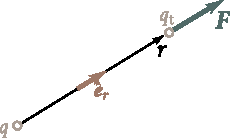
\includegraphics[scale=1]{figures/ch_01/fig_1_4.pdf}
		\caption[]{}
		\label{fig:1_4}
	\end{center}
	\vspace{-0.8cm}
\end{figure}

Chúng ta sẽ đi tìm hiểu về điện trường gây ra bởi một điện tích cố định $q$, bằng các sử dụng điện tích thử để xác định nó. Chúng ta đặt điện tích thử vào trường, sao cho $\vec{r}$ là vector xác định vị trí của nó đối với điện tích $q$ (\fig{1_4}). Chúng ta thấy rằng, điện tích thử sẽ chịu một lực
\begin{equation}\label{eq:1_13}
	\vec{F} = \ab{q}{t} \parenthesis{
	\frac{1}{4\pi\varepsilon_0} \frac{q}{r^2}\,\vecuni{r}
	}
\end{equation}

\noindent
[xem phương trình \eqref{eq:1_3} và \eqref{eq:1_11}]. Ở đây, $\vecuni{r}$ là vector đơn vị của vector vị trí $\vec{r}$.

Khi nhìn vào \eqn{1_13} chúng ta thấy rằng, lực tác dụng lên điện tích thử không chỉ phụ thuộc vào các đại lượng đặc trưng của trường (là $q$ và $\vec{r}$), nhưng còn phụ thuộc vào độ lớn của điện tích thử $\ab{q}{t}$. Nếu chúng ta xét các điện tích thử $\ab{q}{t}'$,$\ab{q}{t}''$, \ldots, thì lực $\vec{F'}$,$\vec{F''}$, \ldots tương ứng sẽ khác nhau.
Chúng ta có thể thấy từ \eqn{1_13}, rằng tỉ lệ $F/\ab{q}{t}$ cho bất kì một điện tích thử nào đều như nhau, và tỉ lệ này chỉ phụ thuộc vào đại lượng  $q$ và $\vec{r}$. Vì thế, nó sẽ trở nên tự nhiên hơn nếu chúng ta sử dụng tỉ lệ này đại lượng để xác định điện trường:
\begin{equation}\label{eq:1_14}
	\vec{E} = \frac{\vec{F}}{\ab{q}{t}}.
\end{equation}

\noindent
Đại lượng vector này được gọi là \textbf{cường độ điện trường} (hay \textbf{độ mạnh điện trường}) tại một điểm xác định (hay tại một điểm mà điện tích thử $\ab{q}{t}$ chịu một lực $\vec{F}$).

Theo \eqn{1_14}, cường độ điện trường bằng với lực tác dụng lên một đơn vị điện tích, tại một vị trí xác định. Hướng của vector $\vec{E}$ sẽ trùng với hướng của lực nếu điện tích thử dương, còn nếu điện tích thử là âm thì ngược lại.

Cần lưu ý rằng \eqn{1_14} vẫn đúng cho trường hợp điện tích thử âm ($\ab{q}{t}<0$). Trong trường này, vector $\vec{E}$ và vector $\vec{F}$ ngược hướng.

Chúng ta đã tiếp cận với ý tưởng về cường độ điện trường khi nghiên cứu về một điện tích điểm cố định. Nhưng định nghĩa về $\vec{E}$ trong \eqref{eq:1_14} cũng đúng cho trường hợp hệ gồm nhiều điện tích. Tuy nhiên, chúng ta cần phải lưu ý vài chỗ. Các điện tích trong một hệ sẽ bị phân bố lại dưới sự tác dụng của điện tích thử. Điều này là hoàn toàn có thể xảy ra, ví dụ, điện tích của hệ nằm trong một vật dẫn. Mặt khác các điện tích này có thể chuyển động tự do trong vật dẫn. Để tránh sự phân bố lại điện tích trong hệ, ta sẽ sử dụng một điện tích thử có giá trị vô cùng bé.

Theo \eqref{eq:1_13} và \eqref{eq:1_14}, cường độ điện trường tạo ra bởi một điện tích điểm tỉ lệ thuận với độ lớn của $q$ và tỉ lệ nghịch với bình phương khoảng cách $r$ từ điện tích đến điểm đang xét:
\begin{equation}\label{eq:1_15}
	\vec{E} = \frac{1}{4\pi\varepsilon_0} \frac{q}{r^2}\, \vecuni{r}.
\end{equation}

\noindent
Vector $\vec{E}$ nằm dọc trên đường thẳng chứa điện tích và điểm đang xét trong trường. Nó có hướng từ điện tích đi ra xa nếu điện tích dương, và có hướng từ xa vô cùng đến điện tích nếu điện tích âm.

Trong hệ Gauss, phương trình cho cường độ điện trường của một điện tích điểm trong chân không có dạng là:
\begin{equation}\label{eq:1_16}
	\vec{E} = \frac{q}{r^2}\, \vecuni{r}.
\end{equation}

Đơn vị của cường độ điện trường là cường độ tại một điểm mà có một đơn vị lực (\SI{1}{\newton} trong hệ SI và \SI{1}{\dyne} trong hệ Gauss) tác dụng lên một đơn vị điện tích (\SI{1}{\coulomb} trong hệ SI và \num{1}\cgse{q} trong hệ Gauss). Đơn vị của cường độ điện trường không có tên riêng trong hệ Gauss. Trong hệ SI thì nó có đơn vị là volt trên mét (\si{\volt\per\metre}) [xem \eqn{1_44}].

Theo \eqn{1_15}, một điện tích \SI{1}{\coulomb} sẽ tạo ra một cường độ điện trường trong chân không tại một điểm cách nó một khoảng \SI{1}{\metre} là:
\begin{equation*}
	E = \frac{1}{4\pi\parenthesis{1/4\pi \times \num{9e9}}} \frac{1}{1^2} = \SI{9e9}{\volt\per\metre}.
\end{equation*}

Xét trong hệ Gauss ta có
\begin{equation*}
	E = \frac{q}{r^2} = \frac{\num{3e9}}{100^2} = \num{3e5}\cgse{E}.
\end{equation*}

\noindent
So sánh hai đáp án trên ta có:
\begin{equation}\label{eq:1_17}
	1\cgse{E} = \SI{3e4}{\volt\per\metre}.
\end{equation}

Theo \eqn{1_14}, lực tác dụng lên điện tích thử là
\begin{equation*}
	\vec{F} = \ab{q}{t} \vec{E}.
\end{equation*}

\noindent
Dễ dàng thấy rằng, bất kì điện tích điểm $q$\footnote{Trong \eqn{1_15}, $q$ là điện tích thiết lập nên trường. Trong \eqn{1_18}, $q$ là điện tích chịu tác dụng của lực $\vec{F}$ tại điểm có cường độ $\vec{E}$.} nào được đặt tại điểm có cường độ điện trường $\vec{E}$, sẽ chịu một lực
\begin{equation}\label{eq:1_18}
	\vec{F} = q \vec{E}.
\end{equation}

\noindent
Nếu điện tích $q$ dương, thì hướng của lực sẽ trùng với hướng của vector $\vec{E}$. Ngược lại, nếu $q$ âm, thì vector $\vec{F}$ sẽ ngược chiều $\vec{E}$.

Chúng ta đã đề cập đến ở \sect{1_2}, rằng lực gây ra bởi một hệ các điện tích sẽ bằng tổng hợp vector lực của từng thành phần trong hệ [xem \eqn{1_15}]. Do đó, nó sẽ đúng khi phát biểu \textit{điện trường gây ra bởi hệ các điện tích, tại một điểm nào đó, sẽ bằng tổng hợp vector điện trường của từng thành phần trong hệ}:
\begin{equation}\label{eq:1_19}
	\vec{E} = \sum_i \vec{E}_i.
\end{equation}

\noindent
Nhận định này được gọi là \textbf{nguyên lý chồng chất điện trường}

Nguyên lý chồng chất cho phép chúng ta tính toán điện trường của một hệ điện tích bất kì. Bằng cách chia nhỏ vật thể nhiễm điện thành những thành phần $\deriv{q}$ rất nhỏ, chúng ta sẽ biến hệ điện tích thành một tập hợp các điện tích điểm. Sau đó, chúng ta chỉ cần tính toán tác dụng của từng điện tích đó lên điểm đang xét theo \eqn{1_15}

Điện trường có thể mô tả qua việc xác định độ lớn và hướng của vector $\vec{E}$ tại một điểm. Tổng hợp những vector này lại sẽ tạo nên một trường vecor cường độ điện trường (so sánh với trường vector vận tốc, Vol. I, Sec. 9.1). Trường vector vận tốc được mô tả bằng các đường dòng. Tương tự, đối với điện trường, chúng ta cũng có thể mô tả nó dưới dạng các đường dòng, mà chúng ta có thể gọi ngắn gọn là đường sức điện. Mật độ đường sức bằng với số đường sức đi qua một đơn vị diện tích (vuông góc với $\vec{E}$), và nó có giá trị bằng với độ lớn của vector $\vec{E}$. Do đó, hình dạng của đường sức cho phép chúng ta xác định được độ lớn và hướng của $\vec{E}$ tại một điểm bất kì (\fig{1_5}).

\begin{figure}[!htb]
	\begin{minipage}[t]{0.5\linewidth}
		\begin{center}
			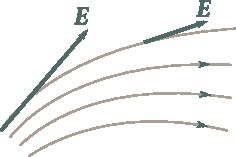
\includegraphics[scale=1]{figures/ch_01/fig_1_5.pdf}
			\caption[]{}
			\label{fig:1_5}
		\end{center}
	\end{minipage}
	\hspace{-0.05cm}
	\begin{minipage}[t]{0.5\linewidth}
		\begin{center}
			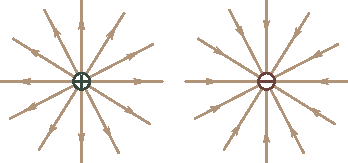
\includegraphics[scale=1]{figures/ch_01/fig_1_6.pdf}
			\caption[]{}
			\label{fig:1_6}
		\end{center}
	\end{minipage}
\vspace{-0.4cm}
\end{figure}

Đường sức của một điện tích điểm là các đường thẳng xuyên tâm, có hướng đi ra xa khỏi điện tích (nếu nó dương), hoặc hướng vào điện tích (nếu nó âm). Điện tích là một đầu mút của đường sức, đầu mút còn lại thì ở xa vô cùng. Chúng ta có, tổng đường sức xuyên qua một mặt cầu có bán kính $r$ sẽ bằng với tích của mật độ đường sức với diện tích bề mặt của mặt cầu $4\pi r^2$. Cho rằng mật độ đường sức có giá trị đại số là $E=(1/4\pi\varepsilon_0)(q/r^2)$. Vì thế, ta có số đường sức xuyên qua toàn bộ mặt cầu là $(1/4\pi\varepsilon_0)(q/r^2) 4\pi r^2=q/\varepsilon_0$. Kết quả này cho ta thấy rằng tổng số đường sức điện xuyên qua một mặt bao quanh điện tích là như nhau. Chúng ta cũng có thể suy ra rằng, các đường sức luôn có một đầu mút là điện tích, và đường sức sẽ hướng từ điện tích ra xa (nếu điện tích dương) hoặc hướng từ vô cùng về điện tích (nếu điện tích âm). Tính chất này của đường sức điện là cơ bản trong trường tĩnh điện, hay đường sức của một hệ điện tích cố định chỉ có thể bắt đầu, và kết thúc duy nhất tại ngay điện tích.

\section{Điện Thế}\label{sec:1_6}

Chúng ta cùng xem xét trường điện trường gây ra bởi một điện tích điểm cố định $q$. Tại một điểm bất kì trong trường, điện tích $q'$ sẽ chịu một lực
\begin{equation}\label{eq:1_20}
	\vec{F} = \frac{1}{4\pi\varepsilon_0}\frac{qq'}{r^2}\, \vecuni{r} = F(r)\vecuni{r}.
\end{equation}

\noindent
Ở đây $F(r)$ là độ lớn của lực $\vec{F}$, $\vec{r}$ là vector giúp xác định vị trí của $q'$ so với $q$, có vector đơn vị là $\vecuni{r}$.

\begin{figure}[!htb]
	\begin{center}
		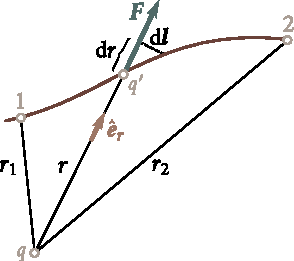
\includegraphics[scale=1]{figures/ch_01/fig_1_7.pdf}
		\caption[]{}
		\label{fig:1_7}
	\end{center}
	\vspace{-0.8cm}
\end{figure}

Lực trong \eqref{eq:1_20} là một lực xuyên tâm (xem Vol. I, Sec. 3.4). Trường xuyên tâm có tính bảo toàn. Vì thế, công của điện trường tác dụng lên điện tích $q'$ khi di chuyển từ một điểm đến một vị trí khác là không phụ thuộc vào hình dạng đường đi. Công này được tính là:
\begin{equation}\label{eq:1_21}
	A_{12} = \int_1^2 F(r) \vecuni{r}\, \deriv{\vec{l}}
\end{equation}

\noindent
Trong đó $\deriv{\vec{l}}$ là độ dời nguyên tố của điện tích $q'$. Hình \fig{1_7} cho chúng ta thấy rằng tích vô hướng của $\vecuni{r}\,\deriv{\vec{l}}$ bằng với biến thiên độ lớn của vector $\vec{r}$, hay $\deriv{r}$. Phương trình \eqref{eq:1_21} có thể được viết dưới dạng
\begin{equation*}
	A_{12} = \int_1^2 F(r)\, \deriv{r}
\end{equation*}

\noindent
[so sánh với phương trình (3.24) của Vol. I]. Sử dụng biểu thức của $F(r)$ ta sẽ có:
\begin{equation}\label{eq:1_22}
	A_{12} = \frac{qq'}{4\pi\varepsilon_0} \int_{r_1}^{r_2} \frac{\deriv{r}}{r^2} = \frac{1}{4\pi\varepsilon_0} \parenthesis{
	\frac{qq'}{r_1} - \frac{qq'}{r_2}
	}.
\end{equation}

Công của một trường bảo toàn có thể được biểu diễn dưới dạng biến thiên thế năng:
\begin{equation}\label{eq:1_23}
	A_{12} = \ab{W}{p,$1$} - \ab{W}{p,$2$}.
\end{equation}

\noindent
So sánh giữa phương trình \eqref{eq:1_22} và \eqref{eq:1_23}, ta thấy rằng thế năng của $q'$ trong điện trường của $q$ còn có thể được biểu diễn là:
\begin{equation*}
	\ab{W}{p} = \frac{1}{4\pi\varepsilon_0} \frac{qq'}{r_2} + \text{constant}.
\end{equation*}

\noindent
Giá trị của hằng số trong phương trình trên thường được chọn là thế năng ở vô cùng (tức là $r=\infty$), ở đó thế năng bị triệt tiêu.
\begin{equation}\label{eq:1_24}
	\ab{W}{p} = \frac{1}{4\pi\varepsilon_0} \frac{qq'}{r_2}.
\end{equation}

Chúng ta sử dụng điện tích $q'$ như là một điện tích thử để nghiên cứu về điện trường. Theo \eqn{1_24}, thế năng không chỉ phụ thuộc vào độ lớn của $q'$, nhưng còn phụ thuộc vào các đại lượng của trường như $q$ và $r$. Vì thế, chúng ta có thể sử dụng thế năng để mô tả điện trường, tương tự cách chúng ta dùng lực.

Với mỗi điện tích thử khác nhau $\ab{q}{t}'$, $\ab{q}{t}''$, \ldots, sẽ có những thế năng khác nhau $\ab{W}{p}'$, $\ab{W}{p}''$, \ldots, tại cùng một vị trí đang xét. Tuy nhiên, tỉ lệ $\ab{W}{p}/\ab{q}{t}$ luôn không đổi đối với mọi điện tích thử [xem \eqn{1_24}].
\begin{equation}\label{eq:1_25}
	\varphi = \frac{\ab{W}{p}}{\ab{q}{t}}
\end{equation}

\noindent
thường được sử dụng cùng với cường độ điện trường $\vec{E}$ nhằm mô tả điện trường.

Có thể thấy từ \eqn{1_25} rằng, điện thế có giá trị đại số bằng với thế năng tại một điểm xác định của một đơn vị điện tích dương. Thay thế năng vào \eqn{1_25}, chúng ta sẽ tính được giá trị của điện thế do một điện tích gây ra.
\begin{equation}\label{eq:1_26}
	\varphi = \frac{1}{4\pi\varepsilon_0} \frac{q}{r}.
\end{equation}

Trong hệ thống Gauss, điện thế của một điện tích điểm trong chân không được xác định bởi công thức
\begin{equation}\label{eq:1_27}
	\varphi = \frac{q}{r}.
\end{equation}

Chúng ta cùng xem xét điện trường tạo bởi $N$ điện tích điểm $q_1, q_2,\ldots, q_N$. Ta cho $r_1, r_2,\ldots, r_N$ lần lượt là khoảng cách từ các điện tích đến điểm đang xét. Công thực hiện bởi trường tổng hợp lên $q'$ này sẽ bằng tổng đại số các công của từng điện tích trong hệ:
\begin{equation*}
	A_{12} = \sum_{i=1}^N A_i.
\end{equation*}

\noindent
Theo \eqn{1_22}, công $A_i$ được tính là:
\begin{equation*}
	A_{i} = \frac{1}{4\pi\varepsilon_0} \parenthesis{
	\frac{q_i q'}{r_{i,1}} - \frac{q_i q'}{r_{i,2}}
	}
\end{equation*}

\noindent
Ở đây, $r_{i,1}$ là khoảng cách từ điện tích $q_i$ đến vị trí ban đầu của $q'$, và $r_{i,2}$ là khoảng cách từ $q_i$ đến vị trí cuối cùng của $q'$. Do đó,
\begin{equation*}
	A_{i2} = \frac{1}{4\pi\varepsilon_0} \sum_{i=1}^N \frac{q_i q'}{r_{i,1}} - \frac{1}{4\pi\varepsilon_0} \sum_{i=1}^N \frac{q_i q'}{r_{i,2}}.
\end{equation*}

\noindent
So sánh phương trình này với \eqn{1_23}, chúng ta sẽ có được thế năng của $q'$ trong điện trường tạo ra bởi một hệ các điện tích:
\begin{equation*}
	\ab{W}{p} = \frac{1}{4\pi\varepsilon_0} \sum_{i=1}^N \frac{q_i q'}{r_{i}}
\end{equation*}

\noindent
Do đó ta có
\begin{equation}\label{eq:1_28}
	\varphi = \frac{1}{4\pi\varepsilon_0} \sum_{i=1}^N \frac{q_i}{r_{i}}.
\end{equation}

So sánh công thức này với \eqn{1_26}, chúng ta sẽ đi đến được kết luận rằng \textit{điện thế của một hệ điện tích bằng với tổng đại số điện thế của từng thành phần trong hệ}. Nếu cường độ điện trường của một hệ là tổng hợp vector các điện trường thành phần trong hệ, thì điện thế sẽ là tổng đại số. Điều này cho ta thấy rằng, tính toán điện thế thường dễ dàng so với điện trường.

Xem xét lại \eqn{1_25}, chúng ta thấy rằng một điện tích $q$ tại một điểm trong điện trường có điện thế $\varphi$ sẽ có thế năng:
\begin{equation}\label{eq:1_29}
	\ab{W}{p} = q\varphi.
\end{equation}

\noindent
Do đó, công của trường tác dụng lên điện tích $q$ có thể được biểu diễn dưới dạng biến thiên thế năng.
\begin{equation}\label{eq:1_30}
	A_{12} = \ab{W}{p,$1$} - \ab{W}{p,$2$} = q \parenthesis{\varphi_1 - \varphi_2}.
\end{equation}

\noindent
Thật vậy, công thực hiện lên điện tích của điện trường bằng với tích của độ lớn điện tích với hiệu điện thế giữa điểm đầu và cuối (hay độ giảm điện thế).

Nếu điện tích $q$ bị dời từ một điểm có điện thế $\varphi$ đến vô cùng (nơi mà ta quy ước điện thế bằng 0), thì công của trường tác dụng lên điện tích là:
\begin{equation}\label{eq:1_31}
	A_{\infty} = q \varphi.
\end{equation}

\noindent
Do đó, điện thế có giá trị đại số bằng với công để dời một đơn vị điện tích dương ra xa vô cùng. Để đưa một đơn vị điện tích dương từ vô cùng về điểm đó, thì ta phải tác dụng một công có cùng độ lớn nhưng ngược dấu với công do lực điện gây ra.

Phương trình \eqref{eq:1_31} có thể dùng để thành lập đơn vị của điện thế. Điện thế được định nghĩa là công tác dụng lên một đơn vị điện tích dương để đưa nó từ vô cùng về một điểm cho trước. Đơn vị SI của điện thế là volt (\si{\volt}), được định nghĩa là điện thế tại điểm mà cần thực hiện một công $1$ joule để dời một điện tích $1$ coulomb từ vô cùng về điểm đó.
\begin{equation}\label{eq:1_32}
	\SI{1}{\joule} = \SI{1}{\coulomb} \times \SI{1}{\volt},\quad  \text{thus,}\quad \SI{1}{\volt} = \frac{\SI{1}{\joule}}{\SI{1}{\coulomb}}.
\end{equation}

Đơn vị tĩnh điện tuyệt đối của điện thế (\cgse{\varphi}) được định nghĩa là điện thế tại một điểm mà cần thực hiện một công \SI{1}{\erg} để đưa một điện tích \num{+1}\cgse{q}, từ vô cùng trở về điểm đó. Thay giá trị \SI{1}{\joule} và \SI{1}{\coulomb} vào \eqn{1_32}, ta sẽ tìm được liên hệ giữa đơn vị volt và đơn vị cgse của điện thế:
\begin{equation}\label{eq:1_33}
	\SI{1}{\volt} = \frac{\SI{1}{\joule}}{\SI{1}{\coulomb}} = \frac{\SI{e7}{\erg}}{\num{3e9}\cgse{q}} = \frac{1}{300}\cgse{\varphi}.
\end{equation}

\noindent
Thus, $1$\cgse{\varphi} equals \SI{300}{\volt}. Do đó, $1$\cgse{\varphi} bằng \SI{300}{\volt}.

Đơn vị của năng lượng và công được gọi là \textbf{electron-volt} (\si{\electronvolt}, được sử dụng thường xuyên trong vật lý. Một electron-volt được định nghĩa là công của trường tác dụng lên một electron (hay điện tích nguyên tố $e$), nếu nó có hiệu điện thế là \SI{1}{\volt}:
\begin{equation}\label{eq:1_34}
	\SI{1}{\electronvolt} = \SI{1.60e-19}{\coulomb} \times \SI{1}{\volt} = \SI{1.60e-19}{\joule} = \SI{1.60e-12}{\erg}.
\end{equation}

\noindent
Những đơn vị thường được sử dụng của electron-volt là:
\begin{align*}
	\text{\SI{1}{\kilo\electronvolt} (kiloelectron-volt)} &= \SI{e3}{\electronvolt},\\
	\text{\SI{1}{\mega\electronvolt} (megaelectron-volt)} &= \SI{e6}{\electronvolt},\\
	\text{\SI{1}{\giga\electronvolt} (gigaelectron-volt)} &= \SI{e9}{\electronvolt}.
\end{align*}

\section{Thế Năng Tương Tác của một Hệ Điện Tích}\label{sec:1_7}

Phương trình \eqref{eq:1_24} biểu diễn thế năng chung của hệ điện tích $q$ và $q'$. Ta kí hiệu các điện tích lần lượt là $q_1$ và $q_2$, ta sẽ có công thức tính thế năng tương tác
\begin{equation}\label{eq:1_35}
	\ab{W}{p} = \frac{1}{4\pi\varepsilon_0} \frac{q_1q_2}{r_{12}}.
\end{equation}

\noindent
Đại lượng $r_{12}$ là khoảng cách giữa các điện tích với nhau.

Ta xét một hệ gồm $N$ hạt điện tích $q_1, q_2, \ldots, q_N$. Chúng ta đã đề cập ở Sec. 3.6 của Vol. I, thế năng tương tác của một hệ bằng tổng đại số thế năng tương tác của từng cặp.
\begin{equation}\label{eq:1_36}
	\ab{W}{p} = \frac{1}{2} \sum_{(i\neq k)} \ab{W}{p,$ik$}(r_{ik})
\end{equation}

\noindent
[xem phương trình (3.60) của Vol. I]

Theo \eqn{1_35}
\begin{equation*}
	\ab{W}{p,$ik$} = \frac{1}{4\pi\varepsilon_0} \frac{q_i q_k}{r_{ik}}.
\end{equation*}

\noindent
Using this equation in \eqref{eq:1_36}, we find that Sử dụng phương trình \eqref{eq:1_36}, chúng ta có thể thấy:
\begin{equation}\label{eq:1_37}
	\ab{W}{p} = \frac{1}{2} \sum_{(i\neq k)} \frac{1}{4\pi\varepsilon_0} \frac{q_i q_k}{r_{ik}}.
\end{equation}

Trong hệ Gauss, đại lượng $1/(4\pi\varepsilon_0)$ được coi bằng $1$ trong phương trình này.

Trong \eqn{1_37}, biểu thức được biểu diễn dưới dạng tổng của chỉ số dưới $i$ và $k$. Các chỉ số $i$ và $k$ có giá trị lần lượt từ $1$ đến $N$. Lưu ý là biểu thức sẽ không bao gồm các hạng tử có $i$ trùng với $k$. Từ đấy ta viết được 
\begin{equation}\label{eq:1_38}
	\ab{W}{p} = \frac{1}{2} \sum_{i=1}^N q_i \sum_{\substack{{i=1}\\ (i\neq k)}}^N \frac{1}{4\pi\varepsilon_0} \frac{q_k}{r_{ik}}.
\end{equation}

\noindent
Còn biểu thức
\begin{equation*}
	\varphi_i =  \frac{1}{4\pi\varepsilon_0} \sum_{\substack{{i=1}\\ (i\neq k)}}^N \frac{q_k}{r_{ik}}
\end{equation*}

\noindent
là điện thế tại vị trí của $q_i$ và được tạo ra bởi những điện tích khác trong hệ, ngoại trừ chính nó. Theo đó, chúng ta có được phương trình để tính thế năng tương tác là:
\begin{equation}\label{eq:1_39}
	\ab{W}{p} = \frac{1}{2} \sum_{i=1}^N q_i \varphi_i.
\end{equation}

\section{Liên Hệ Giữa Cường Độ Điện Trường và Điện Thế}\label{sec:1_8}

Điện trường có thể được mô tả bằng đại lượng vector $\vec{E}$, hoặc với đại lượng vô hướng $\varphi$. Chắc chắn có sự liên hệ giữa hai đại lượng trên. Nếu $\vec{E}$ tỉ lệ thuận với lực tác dụng lên một điện tích nào đó, và $\varphi$ tỉ lệ thuận với thế năng của điện tích tại một vị trí xác định. Như thế liên hệ giữa cường độ điện trường và điện thế, giống như liên hệ của lực với thế năng.

Liên hệ của $\vec{F}$ và thế năng được biểu diễn là:
\begin{equation}\label{eq:1_40}
	\vec{F} = -\nabla\ab{W}{p}
\end{equation}

\noindent
[xem phương trình (3.32) của Vol. I]. Với một hạt điện tích trong trường tĩnh điện, chúng ta có $\vec{F}=q\vec{E}$ và $\ab{W}{p}=q\varphi$. Những điều này đã được nói đến ở \eqn{1_40}. Chúng ta có rằng:
\begin{equation*}
	q \vec{E} = -\nabla(q\varphi).
\end{equation*}

\noindent
Hằng số $q$ có thể được đưa ra khỏi dấu gradient. Chúng ta có thể triệt tiêu $q$, và ta sẽ có công thức
\begin{equation}\label{eq:1_41}
	\vec{E} = -\nabla\varphi
\end{equation}

\noindent
đây liên hệ giữa cường độ điện trường và điện thế.

Sử dụng định nghĩa của gradient [xem phương trình (3.31) của Vol. I], chúng ta có thể ghi là
\begin{equation}\label{eq:1_42}
	\vec{E} = -\diffpartial{\varphi}{x}\vecuni{x} -\diffpartial{\varphi}{y}\vecuni{y} -\diffpartial{\varphi}{z}\vecuni{z}.
\end{equation}

\noindent
\eqn{1_42} khi được chiếu lên các trục toạ độ là:
\begin{equation}\label{eq:1_43}
	E_x = -\diffpartial{\varphi}{x},\quad E_y = -\diffpartial{\varphi}{y},\quad E_z = -\diffpartial{\varphi}{z}.
\end{equation}

\noindent
Tương tự, hình chiếu của vector $\vec{E}$ lên một phương $l$ xác định bằng với đạo hàm của $\varphi$ theo $l$, trong đó dấu trừ thể hiện cho độ giảm của điện thế khi di chuyển theo hướng của $l$.   
\begin{equation}\label{eq:1_44}
	E_l = -\diffpartial{\varphi}{l}.
\end{equation}

\noindent
Có thể thấy rằng việc chọn $l$ là một trục toạ độ, khi áp dụng \eqn{1_43} vào \eqn{1_44}, là việc đúng đắn.

Giờ chúng ta sẽ đi giải thích \eqn{1_41} qua một ví dụ về điện trường của điện tích điểm. Điện thế của trường hợp này được biểu diễn ở \eqn{1_26}. Áp dụng hệ toạ độ Cartesian, ta có cách biểu diễn sau
\begin{equation*}
	\varphi = \frac{1}{4\pi\varepsilon_0} \frac{q}{r} = \frac{1}{4\pi\varepsilon_0} \frac{q}{\parenthesis{x^2 + y^2 + z^2}^{1/2}}.
\end{equation*}

\noindent
Đạo hàm riêng của hàm số này theo biến $x$ là
\begin{equation*}
	\diffpartial{\varphi}{x} = -\frac{1}{4\pi\varepsilon_0} \frac{qx}{\parenthesis{x^2 + y^2 + z^2}^{3/2}} = -\frac{1}{4\pi\varepsilon_0} \frac{qx}{r^3}.
\end{equation*}

\noindent
Tương tự,
\begin{equation*}
	\diffpartial{\varphi}{y} = -\frac{1}{4\pi\varepsilon_0} \frac{qy}{r^3},\quad \diffpartial{\varphi}{y} = -\frac{1}{4\pi\varepsilon_0} \frac{qz}{r^3}.
\end{equation*}

\noindent
Sử dụng các biểu thức đạo hàm đã tính được ở trên, thay vào thì ta có
\begin{equation*}
	\vec{E} = \frac{1}{4\pi\varepsilon_0} \frac{q \parenthesis{x\vecuni{x}+y\vecuni{y}+z\vecuni{z}}}{r^3} = \frac{1}{4\pi\varepsilon_0} \frac{q\vec{r}}{r^3} = \frac{1}{4\pi\varepsilon_0} \frac{q}{r^2}\,\vecuni{r}
\end{equation*}

\noindent
nó tương đương với \eqn{1_15}

Phương trình \eqref{eq:1_41} cho phép chúng ta tìm điện trường tại một điểm đã biết giá trị $\varphi$. Chúng ta có thể tính ngược lại, nếu có giá trị điện trường $\vec{E}$ tại một điểm, thì ta có thể tính ra điện thế. Để tính được điện thế từ điện trường, chúng ta sẽ đi tính công thực hiện bởi lực điện khi dịch chuyển điện tích $q$ từ điểm $1$ đến đến điểm $2$.
\begin{equation*}
	A_{12} = \int_1^2 q \vec{E}\, \deriv{\vec{l}}.
\end{equation*}

\noindent
Mặt khác, theo \eqn{1_30}, công này còn được viết là
\begin{equation*}
	A_{12} = q \parenthesis{\varphi_1 - \varphi_2}.
\end{equation*}

\noindent
Đồng nhất hai biểu thức trên và triệt tiêu $q$, chúng ta sẽ có
\begin{equation}\label{eq:1_45}
	\varphi_1 - \varphi_2 = \int_1^2 \vec{E}\, \deriv{\vec{l}}.
\end{equation}

\noindent
Tích phân được lấy dọc theo đường bất kì nối giữa điểm $1$ và $2$ do công của trường điện gây ra không phụ thuộc vào đường đi. Với một đường cong kín, $\varphi_1=\varphi_2$, và \eqn{1_45} trở thành
\begin{equation}\label{eq:1_46}
	\oint \vec{E}\, \deriv{\vec{l}} = 0
\end{equation}

\noindent
(hình tròn ở giữa dấu tích phân ám chỉ tích phân này được lấy trên một vòng kín). Chúng ta cần lưu ý rằng, liên hệ này chỉ đúng cho trường tĩnh điện. Chúng ta sẽ thấy ở những trang sau, rằng trường của điện tích động (hay trường thay đổi theo thời gian) không phải là trường thế. Vì thế, điều kiện trong \eqref{eq:1_46} không đúng cho trường không là trường thế.

Mặt đẳng thế là bề mặt gồm những điểm có điện thế như nhau.
\begin{equation*}
	\varphi(x,y,z) = \text{constant}.
\end{equation*}

\noindent
Điện thế dọc theo đoạn $\deriv{l}$ trên bề mặt đẳng thế là không đổi ($\deriv{\varphi}=0$). Mặt khác, theo phương trình \eqn{1_44}, thành phần tiếp tuyến của vector $\vec{E}$ với bề mặt bằng không. Vì thế chúng ta có thể nói rằng, vector $\vec{E}$ xuyên thẳng góc với mặt đẳng thế tại một điểm bất kì. Cần nhớ rằng, vector $\vec{E}$ dọc theo đường tiếp tuyến với đường sức $\vec{E}$. Từ đó chúng ta có thể dễ dàng thấy rằng, đường sức điện trường trực giao (vuông góc) với mọi điểm trên mặt đẳng thế.

Đối với một điểm bất kì, chúng ta có thể vẽ một mặt đẳng thế. Do đó, chúng ta sẽ có vô số các bề mặt. Với hai mặt đẳng thế liền kề, thì độ chênh điện thế giữa hai mặt là giống nhau khi xét hai điểm bất kì thuộc hai bề mặt. Mật độ của các mặt đẳng thế cho phép ta tính toán cường độ điện trường. Mật độ các mặt đẳng thế càng dày đặc, thì điện thế dọc theo phương pháp tuyến bị thay đổi nhanh hơn. Và nếu $\nabla\varphi$ sẽ có giá trị lớn hơn tại điểm đang xét, thì $\vec{E}$ lớn hơn. 

Hình \ref{fig:1_8} cho thấy các mặt đẳng thế (nói một cách chính xác là thiết diện của nó với mặt phẳng giấy) của điện tích điểm. Trong tương quan sự phụ thuộc của $E$ và $r$, mật độ các mặt đẳng thế càng dày đặc khi càng đi gần về điện tích. 

\begin{figure}[!htb]
	\begin{minipage}[t]{0.5\linewidth}
		\begin{center}
			
\includegraphics[scale=1]{figures/ch_01/fig_1_8.pdf}
			\caption[]{}
			\label{fig:1_8}
		\end{center}
	\end{minipage}
	\hspace{-0.05cm}
	\begin{minipage}[t]{0.5\linewidth}
		\begin{center}
			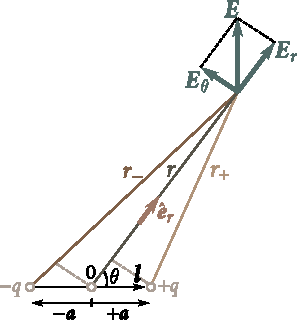
\includegraphics[scale=0.95]{figures/ch_01/fig_1_9.pdf}
			\caption[]{}
			\label{fig:1_9}
		\end{center}
	\end{minipage}
\vspace{-0.4cm}
\end{figure}

Mặt đẳng thế của trường đều là tập hợp các mặt phẳng xếp đều nhau, vuông góc với phương của điện trường.

\section{Lưỡng cực}\label{sec:1_9}

Một \textbf{lưỡng cực điện} được định nghĩa là một hệ hai điện tích điểm $+q$ và $-q$ giống nhau về giá trị và trái dấu, khoảng cách giữa hai điện tích nhỏ hơn rất nhiều so với khoảng cách tới điểm mà trường của hệ đang được quan sát . Đường thẳng đi qua cả hai điện tích gọi là  \textbf{trục lưỡng cực}.

Đầu tiên chúng ta hãy tính điện thế và sau đó là cường độ trường của một lưỡng cực. Trường này có tính đối xứng trục. Do đó, đường sức của trường trong bất kỳ mặt phẳng nào đi qua trục lưỡng cực phải giống nhau, vector $\vec{E}$ nằm trong mặt phẳng này. Vị trí của một điểm so với lưỡng cực được đặc trưng bởi vector vị trí $\vec{r}$ hoặc bởi tọa độ cực $r$ và $\theta$ (\fig{1_9}). Đặt vector $\vec{l}$ có hướng từ điện tích âm tới điện tích dương. Vị trí của điện tích  $+q$ tới tâm của lưỡng cực được xác định bởi vector $\vec{a}$, và của điện tích $-q$ là vector $-\vec{a}$. Hiển nhiên rằng $\vec{l}=2\vec{a}$. Chúng ta sẽ chỉ định khoảng cách tới một điểm cho trước từ $+q$ và $-q$ tương ứng là $r_+$ và $r_-$.

Do $a$ rất nhỏ so với $r$, chúng ta có thể tính xấp xỉ
\begin{equation}\label{eq:1_47}
\begin{split}
	r_+ &= r - a\cos\theta = r - \vec{a}\!\vec{\cdot}\!\vecuni{r},\\
	r_- &= r + a\cos\theta = r + \vec{a}\!\vec{\cdot}\!\vecuni{r}.
\end{split}
\end{equation}

Điện thế tại một điểm xác định bởi vector vị trí $\vec{r}$ là
\begin{equation*}
	\varphi(\vec{r}) = \frac{1}{4\pi\varepsilon_0} \parenthesis{
	\frac{q}{r_+} - \frac{q}{r_-}
	} = \frac{1}{4\pi\varepsilon_0} \frac{q(r_- - r_+)}{r_+ r_-}.
\end{equation*}

\noindent
$r_+r_-$ có thể thay thế bằng $r^2$. Hiệu $r_--r_+$ theo Eqs. \eqref{eq:1_47}, là $2(\vec{a}\!\vec{\cdot}\!\vecuni{r})=\vec{l}\!\vec{\cdot}\!\vecuni{r}$. Từ đó,
\begin{equation}\label{eq:1_48}
	\varphi(\vec{r}) = \frac{1}{4\pi\varepsilon_0} \frac{q(\vec{l}\!\vec{\cdot}\!\vecuni{r})}{r^2} = \frac{1}{4\pi\varepsilon_0} \frac{(\vec{p}\!\vec{\cdot}\!\vecuni{r})}{r^2}
\end{equation}

\noindent
Với
\vspace{-5pt}
\begin{equation}\label{eq:1_49}
	\vec{p} = q\vec{l}
\end{equation}

\noindent
là một đặc trưng của một lưỡng cực gọi là \textbf{moment điện}. vector $\vec{p}$ hướng dọc theo trục lưỡng cực từ điện tích âm tới điện tích dương (\fig{1_10}).

\begin{figure}[!htb]
	\begin{center}
		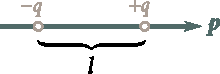
\includegraphics[scale=1]{figures/ch_01/fig_1_10.pdf}
		\caption[]{}
		\label{fig:1_10}
	\end{center}
	\vspace{-0.85cm}
\end{figure}

\eqn{1_48} chỉ ra rằng trường của một lưỡng cực được xác định bởi moment điện của nó $\vec{p}$. Chúng ta sẽ thấy lúc sau rằng biểu hiện của một lưỡng cực trong một điện trường ngoài cũng được xác định bởi moment điện của nó $\vec{p}$. So sánh với \eqn{1_26} chỉ ra rằng điện thế của của một trường lưỡng cực giảm nhanh theo khoảng cách ($1/r^2$) hơn thế năng của một trường điện tích điểm (thay đổi tỷ lệ với $1/r$).

Có thể thấy từ \fig{1_9} rằng $\vec{p}\!\vec{\cdot}\!\vecuni{r}=p\cos\theta$. Do đó, \eqn{1_48} có thể được viết như sau:
\begin{equation}\label{eq:1_50}
	\varphi(r,\theta) = \frac{1}{4\pi\varepsilon_0} \frac{p\cos\theta}{r^2}.
\end{equation}

Để tìm cường độ trường của một lưỡng cực, chúng ta hãy tính hình chiếu của vector $\vec{E}$ theo hai hướng vuông góc với nhau bởi \eqn{1_44}. Một trong số chúng được xác định bởi chuyển động của một điểm do sự thay đổi khoảng cách $r$ (với $\theta$ không đổi), cái còn lại là bởi chuyển động của điểm do thay đổi góc $\theta$ (với $r$ không đổi, xem \fig{1_9}). Hình chiếu đầu tiên nhận được bằng cách vi phân \eqn{1_50} theo $r$:
\begin{equation}\label{eq:1_51}
	E_r = - \diffpartial{\varphi}{r} = \frac{1}{4\pi\varepsilon_0} \frac{2p\cos\theta}{r^3}.
\end{equation}

\noindent
Chúng ta sẽ tìm hình chiếu thứ hai (chúng ta hãy gọi nó là  $E_{\theta}$) bằng cách lấy tỷ lệ giữa sự tăng điện thế $\varphi$ nhận được khi góc $\theta$ tăng một lượng $\deriv{\theta}$ với quãng đường $r\,\deriv{\theta}$ mà ngọn của đoạn $r$ di chuyển được (trong trường hợp này đại lượng $\deriv{l}$ trong \eqn{1_44} bằng với $r\,\deriv{\theta}$). Do đó,
\begin{equation*}
	E_{\theta} = - \frac{1}{r}\diffpartial{\varphi}{\theta}.
\end{equation*}

\noindent
Tính giá trị đạo hàm của hàm số \eqref{eq:1_50} theo $\theta$ ta có
\begin{equation}\label{eq:1_52}
	E_{\theta} = \frac{1}{4\pi\varepsilon_0} \frac{p\sin\theta}{r^3}.
\end{equation}

\noindent
Tổng bình phương của các phương trình \eqref{eq:1_51} và \eqref{eq:1_52} cho ta bình phương của vector $\vec{E}$ (xem \fig{1_9}):
\begin{align*}
	E^2 &= E_r^2 + E_{\theta}^2 = \parenthesis{\frac{1}{4\pi\varepsilon_0}}^2 \parenthesis{\frac{p}{r^3}}^2 \parenthesis{4\cos^2\theta + \sin^2\theta}\\
		&= \parenthesis{\frac{1}{4\pi\varepsilon_0}}^2 \parenthesis{\frac{p}{r^3}}^2 \parenthesis{1 + 3\cos^2\theta}.
\end{align*}

\noindent
Từ đó
\begin{equation}\label{eq:1_53}
	E = \frac{1}{4\pi\varepsilon_0} \frac{p}{r^3} \parenthesis{1 + 3\cos^2\theta}^{1/2}.
\end{equation}

Giả sử trong \eqn{1_53} $\theta=0$, chúng ta được cường độ trên trục lưỡng cực:
\begin{equation}\label{eq:1_54}
	E_{\parallel} = \frac{1}{4\pi\varepsilon_0} \frac{2p}{r^3}.
\end{equation}

\noindent
Vector $\vec{E}_{\parallel}$ hướng dọc theo trục lưỡng cực. Điều này phù hợp với tính đối xứng của bài toán. Kiểm tra \eqn{1_51} chỉ ra rằng $E_r>0$ khi $\theta=0$, và $E_r<0$ khi $\theta=\pi$. Điều này biểu thị rằng trong mọi trường hợp, vector $\vec{E}_{\parallel}$ có hướng trùng với hướng từ $-q$ tới $+q$ (tức là với hướng của $\vec{p}$). Phương trình \eqref{eq:1_54} do đó có thể viết ở dạng vector:
\begin{equation}\label{eq:1_55}
	\vec{E}_{\parallel} = \frac{1}{4\pi\varepsilon_0} \frac{2\vec{p}}{r^3}.
\end{equation}

Giả sử trong \eqn{1_53} $\theta=\pi/2$, chúng ta được cường độ trường trên đường thẳng đi qua tâm lưỡng cực và vuông góc với trục của nó:
\begin{equation}\label{eq:1_56}
	E_{\perp} = \frac{1}{4\pi\varepsilon_0} \frac{p}{r^3}.
\end{equation}

\noindent
Từ \eqn{1_51}, khi $\theta=\pi/2$, hình chiếu $E_r$ bằng không. Từ đó, vector $\vec{E}_{\perp}$ song song với trục lưỡng cực. Từ \eqn{1_52}, khi $\theta=\pi/2$, hình chiếu $E_{\theta}$ là dương. Điều này biểu thị rằng vector $\vec{E}_{\perp}$ hướng theo chiều tăng của góc $\theta$, tức là trực đối với vector $\vec{p}$.

Cường độ trường của một lưỡng cực được đặc trưng bởi sự giảm theo khoảng cách tỷ lệ với $1/r^3$, tức là giảm nhanh hơn so với cường độ trường của một điện tích điểm (giảm tỷ lệ với $1/r^2$).

\begin{figure}[!htb]
	\begin{minipage}[t]{0.5\linewidth}
		\begin{center}
			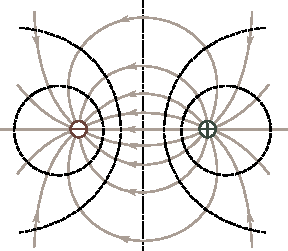
\includegraphics[scale=1]{figures/ch_01/fig_1_11.pdf}
			\caption[]{}
			\label{fig:1_11}
		\end{center}
	\end{minipage}
	\hspace{-0.05cm}
	\begin{minipage}[t]{0.5\linewidth}
		\begin{center}
			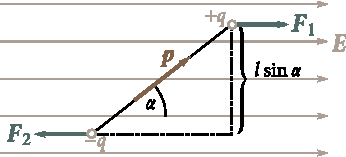
\includegraphics[scale=1]{figures/ch_01/fig_1_12.pdf}
			\caption[]{}
			\label{fig:1_12}
		\end{center}
	\end{minipage}
\vspace{-0.4cm}
\end{figure}

Hình \ref{fig:1_11} cho thấy đường $\vec{E}$ (các đường nét liền) và mặt đẳng thế (các đường nét đứt) của một trường lưỡng cực. Theo \eqn{1_50}, khi $\theta=\pi/2$, điện thế biến mất với mọi $r$. Do đó, mọi điểm thuộc mặt phẳng vuông góc với trục lưỡng cực và đi qua tâm của nó có điện thế bằng không. Điều này có thể dễ đoán bởi vì khoảng cách từ điện tích $+q$ và $-q$ tới bất kì điểm nào thuộc mặt phẳng này là như nhau.

Bây giờ chúng ta hãy xem xét biểu hiện của một lưỡng cực trong một điện trường ngoài. Nếu lưỡng cực được đặt trong một điện trường đều, điện tích $+q$ và $-q$ của lưỡng cực sẽ chịu tác dụng của lực $\vec{F}_1$ và $\vec{F}_2$ có độ lớn bằng nhau, nhưng có hướng ngược nhau (\fig{1_12}). Các lực này tạo thành một cặp có cánh tay đòn là $l\sin\alpha$, tức là phụ thuộc vào định hướng của lưỡng cực trong điện trường. Độ lớn của mỗi lực là $qE$. Nhân nó với cánh tay đòn, chúng ta nhận được độ lớn của moment ngẫu lực tác dụng lên lưỡng cực:
\begin{equation}\label{eq:1_57}
	T = q E l \sin\alpha = p E \sin\alpha
\end{equation}

\noindent
($p$ là moment điện của lưỡng cực). Dễ thấy rằng \eqn{1_57} có thể được viết ở dạng vector
\begin{equation}\label{eq:1_58}
	\vec{T} = \vecprod{p}{E}.
\end{equation}

\noindent
Moment ngẫu lực \eqref{eq:1_58} có khuynh hướng làm quay lưỡng cực sao cho moment điện $\vec{p}$ cùng hướng với trường.

Chúng ta hãy tìm thế năng của lưỡng cực trong điện trường ngoài. Theo \eqn{1_29}, năng lượng này là
\begin{equation}\label{eq:1_59}
	\ab{W}{p} = q\varphi_+ - q\varphi_- = q(\varphi_+ - \varphi_-).
\end{equation}

\noindent
ở đây $\varphi_+$ và $\varphi_-$ là giá trị của điện thế của trường ngoài tại điểm mà $+q$ và $-q$ được đặt.

Điện thế của một trường đều giảm tuyến tính theo hướng của vector $\vec{E}$. Giả sử rằng trục $x$ chỉ hướng này (\fig{1_13}), chúng ta có thể viết $E=E_x=-\diffin{\varphi}{x}$. Xem qua \fig{1_13} chỉ ra rằng hiệu $\varphi_+-\varphi_-$ bằng với độ tăng điện thế trên đoạn $\Delta{x}=l\cos\alpha$:
\begin{equation*}
	\varphi_+ - \varphi_- = \diff{\varphi}{x} l\cos\alpha = -El\cos\alpha.
\end{equation*}

\begin{figure}[!htb]
	\begin{minipage}[t]{0.5\linewidth}
		\begin{center}
			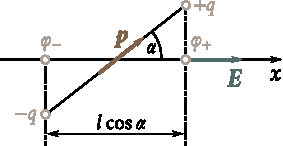
\includegraphics[scale=1]{figures/ch_01/fig_1_13.pdf}
			\caption[]{}
			\label{fig:1_13}
		\end{center}
	\end{minipage}
	\hspace{-0.05cm}
	\begin{minipage}[t]{0.5\linewidth}
		\begin{center}
			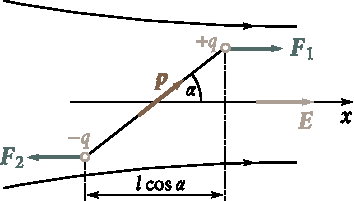
\includegraphics[scale=1]{figures/ch_01/fig_1_14.pdf}
			\caption[]{}
			\label{fig:1_14}
		\end{center}
	\end{minipage}
\vspace{-0.4cm}
\end{figure}

\noindent
Thay giá trị này vào \eqn{1_59}, ta thấy
\begin{equation}\label{eq:1_60}
	\ab{W}{p} = - q E l \cos\alpha = - p E \cos\alpha.
\end{equation}

\noindent
Ở đây $\alpha$ là góc giữa vector $\vec{p}$ và $\vec{E}$. Do đó, chúng ta có thể viết \eqn{1_60} ở dạng
\begin{equation}\label{eq:1_61}
	\ab{W}{p} = - \vecdot{p}{E}.
\end{equation}

\noindent
Chúng ta phải lưu ý rằng biểu thức này không tính đến năng lượng tương tác của các điện tích $+q$ và $-q$ tạo thành lưỡng cực.

Chúng ta đã thu được \eqn{1_61} giả sử đơn giản hóa rằng trường là đều. Tuy nhiên, phương trình này vẫn đúng cho trường không đều.

Chúng ta hãy xét lưỡng cực trong trường không đều đối xứng theo trục $x$\footnote{Một trường hợp cụ thể của một trường như vậy là của một điện tích điểm nếu chúng ta lấy một đường thẳng đi qua điện tích như là trục $x$.}. Hãy đặt tâm của lưỡng cực trên trục này, moment lưỡng cực điện làm với trục một góc $\alpha$, khác $\pi/2$ (\fig{1_14}). Trong trường hợp này, lực tác dụng lên các điện tích lưỡng cực là không giống nhau về độ lớn. Do đó, ngoài moment quay (moment ngẫu lực), lưỡng cực sẽ chịu một lực có xu hướng kéo nó theo hướng của trục $x$. Để tìm giá trị của lực này, chúng ta sử dụng \eqn{1_40}, theo đó
\begin{equation*}
	F_x = -\diffpartial{\ab{W}{p}}{x},\quad F_y = -\diffpartial{\ab{W}{p}}{y},\quad F_z = -\diffpartial{\ab{W}{p}}{z}.
\end{equation*}

\noindent
Theo \eqn{1_60}, có thể viết
\begin{equation*}
	\ab{W}{p}(x,y,z) = -p E(x,y,z)\cos\alpha
\end{equation*}

\noindent
(xem hướng của lưỡng cực so với vector $\vec{E}$ là không đổi, $\alpha=\text{constant}$).

Với các điểm nằm trên trục $x$, đạo hàm của $E$ theo $y$ và $z$ bằng không. Do đó, $\diffinpartial{\ab{W}{p}}{y}=\diffinpartial{\ab{W}{p}}{z}=0$. Vì vậy, Chỉ có thành phần lực $F_x$ khác không. 
\begin{equation}\label{eq:1_62}
	F_x = - \diffpartial{\ab{W}{p}}{x} = p \diffpartial{E}{x} \cos\alpha.
\end{equation}

\noindent
Kết quả này có thể nhận được nếu chúng ta sử dụng sự thật rằng cường độ trường tại các điểm đặt điện tích $+q$ và $-q$ (xem \fig{1_14}) khác một lượng $(\diffinpartial{E}{x})l\cos\alpha$. Theo đó, sự khác biệt giữa các lực tác dụng lên các điện tích là $q(\diffinpartial{E}{x})l\cos\alpha$, giống với \eqn{1_62}.

Khi $\alpha$ nhỏ hơn $\pi/2$, giá trị của $F_x$ xác định bởi \eqn{1_62} là dương. Điều này nói rằng dưới tác dụng của lực thì lưỡng cực bị kéo về vùng có trường mạnh hơn (xem \fig{1_14}). Khi $\alpha$ lớn hơn $\pi/2$, lưỡng cực bị đẩy khỏi trường.

\begin{figure}[!htb]
	\begin{center}
		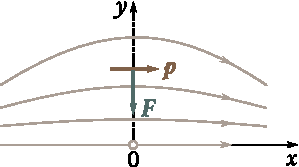
\includegraphics[scale=1]{figures/ch_01/fig_1_15.pdf}
		\caption[]{}
		\label{fig:1_15}
	\end{center}
	\vspace{-0.8cm}
\end{figure}

Ở trường hợp trong \fig{1_15}, chỉ có đạo hàm $\diffinpartial{E}{y}$ khác không cho các điểm trên trục $y$. Do đó, lực tác dụng lên lưỡng cực được xác định bởi thành phần
\begin{equation*}
	F_y = -\diffpartial{\ab{W}{p}}{y} = p \diffpartial{E}{y},\quad (\cos\alpha=1).
\end{equation*}

\noindent
Đạo hàm $\diffinpartial{E}{y}$ âm. Kết quả là, lực có hướng như trong hình. Do đó, trong trường hợp này cũng vậy, lưỡng cực bị kéo về phía trường   .

Lưu ý rằng $-\diffinpartial{\ab{W}{p}}{x}$ cho hình chiếu của lực tác dụng lên hệ theo trục $x$, còn đạo hàm \eqn{1_60} theo $\alpha$ với dấu trừ cho hình chiếu của moment ngẫu lực trên "trục" $\alpha$: $T_{\alpha}=-pE\sin\alpha$. Dấu trừ ở đây là bởi vì "trục" $\alpha$ và moment ngẫu lực $T$ có hướng ngược nhau (xem \fig{1_12}).

\section{Trường của hệ điện tích ở khoảng cách xa}\label{sec:1_10}

Xét hệ $N$ điện tích $q_1, q_2, \ldots, q_N$ trong một thể tích có kích thước $l$, và tìm hiểu về trường tạo ra bởi hệ này tại khoảng cách $r$ rất lớn so với $l$ ($r>l$). Đặt gốc tọa độ $O$ bên trong thể tích chiếm bởi hệ và xác định vị trí của các điện tích bằng các vector vị trí $\vec{r}_i$, (\fig{1_16}; để đơn giản hóa hình ảnh, chúng ta chỉ biểu diễn vector vị trí của điện tích thứ $i$).

\begin{figure}[!htb]
	\begin{center}
		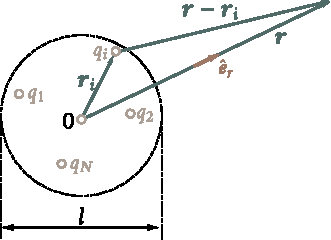
\includegraphics[scale=0.95]{figures/ch_01/fig_1_16.pdf}
		\caption[]{}
		\label{fig:1_16}
	\end{center}
	\vspace{-1.0cm}
\end{figure}

Điện thế tại điểm xác định bởi vector vị trí $\vec{r}$ là
\begin{equation}\label{eq:1_63}
	\varphi(\vec{r}) = \frac{1}{4\pi\varepsilon_0} \sum_{i=1}^N \frac{q_i}{\absolute{\vec{r} - \vec{r}_i}}.
\end{equation}

\noindent
Do $r_i$ rất nhỏ so với $r$, ta có thể cho rằng
\begin{equation*}
	\absolute{\vec{r} - \vec{r}_i} = r - \vec{r}_i\!\vec{\cdot}\!\vecuni{r} = r\parenthesis{1 - \frac{\vec{r}_i\!\vec{\cdot}\!\vecuni{r}}{r}}
\end{equation*}

\noindent
[so sánh với phương trình \eqref{eq:1_47}]. Thay biểu diễn này vào \eqn{1_63} dẫn đến
\begin{equation}\label{eq:1_64}
	\varphi(\vec{r}) = \frac{1}{4\pi\varepsilon_0} \sum_{i=1}^N \frac{q_i}{r} \bracket{\frac{1}{1 - \parenthesis{\vec{r}_i\!\vec{\cdot}\!\vecuni{r}/r}}}.
\end{equation}

\noindent
Sử dụng công thức
\begin{equation*}
	\frac{1}{1-x} \approx 1 + x
\end{equation*}

\noindent
Với $x\ll 1$, ta có thể biến đổi \eqn{1_64} như sau:
\begin{align}
	\varphi(\vec{r}) &= \frac{1}{4\pi\varepsilon_0} \sum_{i=1}^N \frac{q_i}{r} \parenthesis{1 + \frac{\vec{r}_i\!\vec{\cdot}\!\vecuni{r}}{r}}\nonumber\\
	&= \frac{1}{4\pi\varepsilon_0} \frac{1}{r} \sum_{i=1}^N q_i + \frac{1}{4\pi\varepsilon_0} \frac{1}{r^2} \parenthesis{\sum_{i=1}^N q_i \vec{r}_i}\!\vec{\cdot}\!\vecuni{r}. \label{eq:1_65}
\end{align}

\noindent
Số hạng đầu tiên của biểu thức nhận được là điện thế của trường của một điện tích điểm có giá trị $q=\sum_iq_i$ [so sánh với \eqn{1_26}]. Số hạng thứ hai có dạng giống như biểu thức xác định điện thế của một trường lưỡng cực, phần moment điện của lưỡng cực được thay bởi lượng
\begin{equation}\label{eq:1_66}
	\vec{p} = \sum_{i=1}^N q_i \vec{r}_i.
\end{equation}

\noindent
Đại lượng này được gọi là \textbf{moment lưỡng cực điện} của hệ điện tích. Dễ để xác nhận rằng đối với một lưỡng cực \eqn{1_66} biến đổi thành biểu thức $\vec{p}=q\vec{l}$ mà chúng ta đã rất quen thuộc.

\begin{figure}[!htb]
	\begin{minipage}[t]{0.4\linewidth}
		\begin{center}
			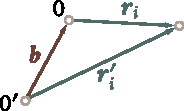
\includegraphics[scale=1]{figures/ch_01/fig_1_17.pdf}
			\caption[]{}
			\label{fig:1_17}
		\end{center}
	\end{minipage}
	\hspace{-0.05cm}
	\begin{minipage}[t]{0.6\linewidth}
		\begin{center}
			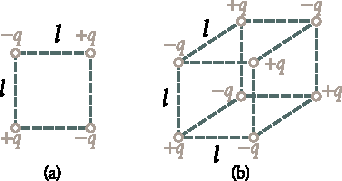
\includegraphics[scale=1]{figures/ch_01/fig_1_18.pdf}
			\caption[]{}
			\label{fig:1_18}
		\end{center}
	\end{minipage}
\vspace{-0.4cm}
\end{figure}

Nếu tổng điện tích của hệ bằng không ($\sum_iq_i=0$), giá trị của moment lưỡng cực không phụ thuộc vào việc chọn gốc tọa độ. Để giải thích việc này, chọn hai gốc tọa độ tùy ý $O$ và $O'$ (\fig{1_17}). Vector vị trí của điện tích thứ $i$ từ các điểm này liên hệ như sau:
\begin{equation}\label{eq:1_67}
	\vec{r}_i' = \vec{b} + \vec{r}_i
\end{equation}

\noindent
(vector $\vec{b}$ như trong hình).Với \eqn{1_67}, moment lưỡng cực trong hệ có gốc $0'$ là
\begin{equation*}
	\vec{p}' = \sum_i q_i \vec{r}_i = \sum_i q_i (\vec{b} + \vec{r}_i) = \vec{b} \sum_i q_i + \sum_i q_i \vec{r}_i.
\end{equation*}

\noindent
Số hạng đầu tiên bằng không (vì $\sum_iq_i=0$). Số hạng thứ hai là $\vec{p}$---moment lưỡng cực trong hệ tọa độ có gốc $O$. Do đó $\vec{p}'=\vec{p}$.

Phương trình \eqref{eq:1_65} về bản chất là hai số hạng đầu tiên của chuỗi khai triển của hàm số \eqref{eq:1_63} thành lũy thừa của $r_i/r$. Khi $\sum_iq_i\neq 0$, số hạng đầu tiên của \eqn{1_65} đóng góp chính vào điện thế (số hạng thứ hai giảm tỷ lệ với $1/r^2$ và do đó nhỏ hơn rất nhiều so với cái đầu tiên). Với một hệ trung hòa điện ($\sum_iq_i=0$), số hạng đầu tiên bằng không, và điện thế được xác định chủ yếu bởi số hạng thứ hai của \eqn{1_65}. Đây là cách mọi việc diễn ra, đặc biệt, cho trường của một lưỡng cực.

Với hệ điện tích mô tả trong \fig{1_18}a được gọi là một \textbf{tứ cực}, cả $\sum_iq_i$ và $\vec{p}$ bằng không, do đó \eqn{1_65} cho điện thế bằng không. Thật ra, trường của một tứ cực, mặc dù nó yếu hơn nhiều so với lưỡng cực (với cùng giá trị của $q$ và $l$), nhưng khác không. Điện thế của trường tạo ra bởi tứ cực được xác định chủ yếu bởi số hạng thứ ba của khai triển tỷ lệ với $1/r^3$. Để nhận được số hạng này, chúng ta phải tính đến đại lượng $(r_i/r)^2$ mà chúng ta đã bỏ qua khi dẫn đến \eqn{1_65}. Với hệ điện tích trong \fig{1_18}b gọi là một \textbf{bát cực}, số hạng thứ ba của khai triển cũng bằng không. Điện thế của trường như vậy được xác định bởi số hạng thứ tư của khai triển, tỷ lệ với $1/r^4$.

Cần lưu ý rằng đại lượng bằng với $\sum_iq_i$ ở tử số của số hạng đầu tiên của \eqn{1_65} được gọi là một \textbf{đơn cực} hoặc một \textbf{đa cực bậc không}, một lưỡng cực cũng được gọi là một \textbf{đa cực bậc một}, một tứ cực được gọi là một \textbf{đa cực bậc hai}, vân vân.

Do đó, trong trường hợp tổng quát, trường của một hệ điện tích tại khoảng cách xa có thể được biểu diễn như là sự chồng chất của các trường tạo bởi đa cực thuộc các cấp khác nhau---đơn cực, lưỡng cực, tứ cực, bát cực, vân vân.

\section{Mô tả các thuộc tính của trường vector}\label{sec:1_11}

Để tiếp tục nghiên cứu điện trường, chúng ta phải làm quen với các công cụ toán học sử dụng để mô tả các tính chất của trường vector. Các công cụ này được gọi là \textbf{phân tích vector}. Trong phần này, ta sẽ xem xét các khái niệm cơ bản và các công thức chọn lọc của phân tích vector, và cũng chứng minh hai định lý chính của nó---định lý Ostrogradsky-Gauss (hoặc là định lý phân kỳ Gauss) và định lý Stokes.

Các đại lượng sử dụng trong phân tích vector có thể được minh họa tốt nhất bởi trường vector vận tốc của chất lỏng đang chảy. Do đó ta đưa ra các đại lượng này khi xử lý với dòng chất lỏng lý tưởng không nén, và sau đó mở rộng kết quả nhận được cho trường vector có bản chất bất kỳ.

Chúng ta đã quen với một trong những khái niệm của phân tích vector. Đó là \textbf{gradient}, sử dụng để mô tả các trường vô hướng. Nếu giá trị của đại lượng vô hướng $\varphi=\varphi(x, y, z)$ gán cho mọi điểm P có tọa độ $x, y, z$, ta nói rằng trường vô hướng của $\varphi$ được thiết lập. Gradient của đại lượng $\varphi$ được định nghĩa là vector
\begin{equation}\label{eq:1_68}
	\grad{\varphi} = \diffpartial{\varphi}{x}\,\vecuni{x} + \diffpartial{\varphi}{y}\,\vecuni{y} + \diffpartial{\varphi}{z}\,\vecuni{z}.
\end{equation}

Độ tăng của hàm $\varphi$ khi dịch chuyển trên chiều dài $\deriv{\vec{l}}=\vecuni{x}\,\deriv{x}+\vecuni{y}\,\deriv{y}+\vecuni{z}\,\deriv{z}$ là
\begin{equation*}
	\deriv{\varphi} = \diffpartial{\varphi}{x}\,\deriv{x} + \diffpartial{\varphi}{y}\,\deriv{y} + \diffpartial{\varphi}{z}\,\deriv{z}
\end{equation*}

\noindent
Có thể viết ở dạng
\begin{equation}\label{eq:1_69}
	\deriv{\varphi} = \grad{\varphi} \ccdot \deriv{\vec{l}}.
\end{equation}

Bây giờ ta sẽ chuyển sang thiết lập các đặc tính của trường vector.

\begin{figure}[!htb]
	\begin{center}
		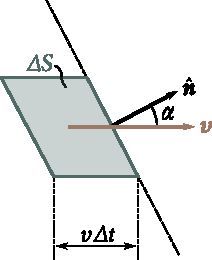
\includegraphics[scale=1]{figures/ch_01/fig_1_19.pdf}
		\caption[]{}
		\label{fig:1_19}
	\end{center}
	\vspace{-0.8cm}
\end{figure}

\textbf{Thông lượng vector.} Giả sử rằng dòng chảy chất lỏng được đặc trưng bởi trường vector vận tốc. Lượng chất lỏng chảy qua một bề mặt tưởng tượng $S$ trong đơn vị thời gian gọi là thông lượng của chất lỏng qua bề mặt này. Để tìm thông lượng, ta chia bề mặt thành các phần nguyên tố có kích thước $\Delta{S}$. Có thể thấy từ \fig{1_19} rằng trong thời gian $\Delta{t}$ lượng chất lỏng bằng
\begin{equation*}
	\Delta{V} = (\Delta{S}\cos\alpha) v\Delta{t}
\end{equation*}

\noindent
sẽ đi qua phần tử $\Delta{S}$. Chia thể tích này với thời gian $\Delta{t}$, ta sẽ tìm được thông lượng qua mặt $\Delta{S}$:
\begin{equation*}
	\Delta{\Phi} = \frac{\Delta{V}}{\Delta{t}} = \Delta{S} v \cos\alpha.
\end{equation*}

\noindent
Chuyển qua vi phân, ta được
\begin{equation}\label{eq:1_70}
	\deriv{\Phi} = (v \cos\alpha)\, \deriv{S}.
\end{equation}

\noindent
Phương trình \eqref{eq:1_70} có thể viết trong hai cách khác nhau. Cách đầu tiên, nếu chúng ta tính đến $v\cos\alpha$ là hình chiếu của vector vận tốc lên pháp tuyến $\vecuni{n}$ của diện tích $\deriv{S}$, ta có thể viết \eqn{1_70} ở dạng
\begin{equation}\label{eq:1_71}
	\deriv{\Phi} = v_n\, \deriv{S}.
\end{equation}

\noindent
Cách thứ hai, ta đưa vào vector $\deriv{\vec{S}}$ có độ lớn bằng diện tích $\deriv{S}$, trong khi hướng của nó trùng với hướng của pháp tuyến $\hatvec{n}$ của diện tích:
\begin{equation*}
	\deriv{\vec{S}} = \deriv{S}\, \hatvec{n}.
\end{equation*}

\noindent
Vì hướng của vector $\hatvec{n}$ được chọn tùy ý (nó có thể là một trong hai bên của diện tích), nên $\deriv{\vec{S}}$ không phải một vector thực, mà là một giả vector. Góc $\alpha$ trong \eqn{1_70} là góc giữa vector $\vec{v}$ và $\deriv{\vec{S}}$. Từ đó, phương trình này có thể được viết ở dạng
\begin{equation}\label{eq:1_72}
	\deriv{\Phi} = \vec{v} \ccdot \deriv{\vec{S}}.
\end{equation}

Bằng cách lấy tổng thông lượng qua tất cả diện tích nguyên tố được chia ra từ bề mặt $S$, ta được thông lượng của chất lỏng qua $S$:
\begin{equation}\label{eq:1_73}
	\Phi_v = \int_S \vec{v} \ccdot \deriv{\vec{S}} = \int_S v_n\, \deriv{S}.
\end{equation}

\noindent
Một biểu thức tương tự cho một trường vector $\vec{a}$ tùy ý, nghĩa là lượng
\begin{equation}\label{eq:1_74}
	\Phi_a = \int_S \vec{a} \ccdot \deriv{\vec{S}} = \int_S a_n\, \deriv{S}
\end{equation}

\noindent
được gọi là \textbf{thông lượng của vector a qua bề mặt} $S$. Theo định nghĩa này, thông lượng của chất lỏng có thể gọi là thông lượng của vector $\vec{v}$ qua bề mặt đã cho [xem \eqn{1_73}].

Thông lượng của một vector là một đại lượng đại số. Dấu của nó phụ thuộc vào việc chọn hướng của pháp tuyến phần tử diện tích được chia ra từ bề mặt $S$ trong tính thông lượng. Đảo hướng của pháp tuyến làm đổi dấu của $a_n$ và, do đó, là dấu của đại lượng \eqref{eq:1_74}. Cách làm thông thường cho mặt kín là tính thông lượng ``hướng ra ngoài'' vùng bên trong bề mặt. Do đó, trong phần sau ta sẽ luôn ngụ ý rằng $\hatvec{n}$ là một ngoại hướng pháp tuyến.

\begin{figure}[!htb]
	\begin{center}
		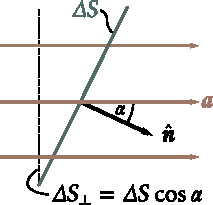
\includegraphics[scale=0.95]{figures/ch_01/fig_1_20.pdf}
		\caption[]{}
		\label{fig:1_20}
	\end{center}
	\vspace{-1.0cm}
\end{figure}

Ta có thể đưa ra một giải thích hình học minh họa cho thông lượng vector. Vì mục đích này, ta sẽ biểu diễn một trường vector bằng một hệ các đường sức $\vec{a}$ được dựng sao cho mật độ các đường sức tại mỗi điểm có trị số bằng với độ lớn của vector $\vec{a}$ tại điểm đó trong trường (so sánh với quy tắc xây dựng các đường sức của vector $\vec{E}$ được nêu ở cuối \sect{1_5}). Ta hãy tìm số giao điểm $\Delta{N}$ của đường sức trường với diện tích ảo $\Delta{S}$. \fig{1_20} chỉ ra rằng số này bằng mật độ đường sức (tức là $a$) nhân với $\Delta{S}_{\perp}=\Delta{S}\cos\alpha$:
\begin{equation*}
	\Delta{N}\, (=)\, a \Delta{S}\cos\alpha = a_n \Delta{S}.
\end{equation*}

\noindent
Ta chỉ nói sự bằng nhau về chỉ số giữa $\Delta{N}$ và $a_n\Delta{S}$. Đó là lý do tại sao dấu bằng nằm trong ngoặc đơn. Theo \eqn{1_74}, biểu thức $a_n\Delta{S}$ là $\Delta{\Phi}$---thông lượng vector qua diện tích $\Delta{S}$. Do đó,
\begin{equation}\label{eq:1_75}
	\Delta{N}\, (=)\, \Delta{\Phi}_a.
\end{equation}

Để dấu của $\Delta{N}$ trùng với dấu của $\Delta{\Phi}_a$, ta phải xem số giao điểm là dương khi góc $\alpha$ giữa chiều dương của đường sức trường và pháp tuyến của diện tích là góc nhọn. Giao điểm được coi là âm nếu góc $\alpha$ là góc tù. Với diện tích trong \fig{1_20}, cả ba giao điểm là dương: $\Delta{N}=+3$ ($\Delta{\Phi}_a$ trong trường hợp này cũng dương vì $a_n>0$). Nếu hướng của pháp tuyến trong \fig{1_20} đảo chiều, giao điểm sẽ trở thành âm ($\Delta{N}=-3$), và thông lượng $\Delta{\Phi}_a$ cũng âm.

Tính tổng của \eqn{1_75} trên bề mặt ảo hữu hạn $S$ dẫn đến
\begin{equation}\label{eq:1_76}
	\Delta{\Phi}_a\, (=)\, \sum\Delta{N} = N_+ - N_-
\end{equation}

\noindent
$N_+$ và $N_-$ lần lượt và tổng số giao điểm dương và âm của đường sức trường với bề mặt $S$.

Người đọc có thể bị rối vì thông lượng được biểu diễn bằng một phân số, số giao điểm của đường trường với bề mặt so với thông lượng cũng sẽ là phân số. Tuy nhiên, đừng nhầm lẫn điều này. Đường sức trường là một hình ảnh có điều kiện bị thiếu đi ý nghĩa vật lý.

Ta hãy lấy một bề mặt tưởng tượng dưới dạng một dải giấy có phần dưới bị xoắn so với phần trên một góc $\pi$ (\fig{1_21}). Hướng của pháp tuyến phải chọn như nhau cho toàn thể bề mặt. Từ đó, nếu ở phần trên của dải, pháp tuyến dương chỉ sang phải, thì pháp tuyến của phần dưới sẽ chỉ sang trái. Theo đó, các giao điểm của đường sức trường miêu tả trong \fig{1_21} với nửa mặt trên là dương, và với nửa dưới là âm.

\begin{figure}[!htb]
	\begin{minipage}[t]{0.4\linewidth}
		\begin{center}
			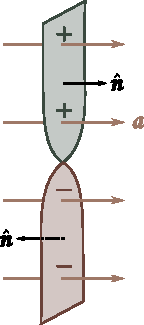
\includegraphics[scale=0.95]{figures/ch_01/fig_1_21.pdf}
			\caption[]{}
			\label{fig:1_21}
		\end{center}
	\end{minipage}
	\hspace{-0.05cm}
	\begin{minipage}[t]{0.6\linewidth}
		\begin{center}
			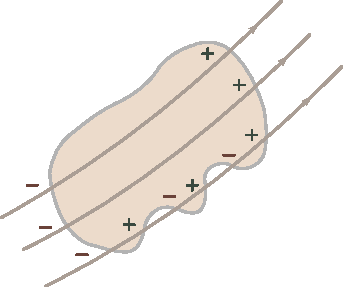
\includegraphics[scale=0.95]{figures/ch_01/fig_1_22.pdf}
			\caption[]{}
			\label{fig:1_22}
		\end{center}
	\end{minipage}
\vspace{-0.4cm}
\end{figure}

Ngoại hướng pháp tuyến được coi là dương với một mặt kín (\fig{1_22}). Do đó, các giao điểm ứng với các điểm mà đường sức đi ra khỏi bề mặt (góc $\alpha$ là góc nhọn) mang dấu dương, và những điểm đường sức đi vào bề mặt (góc $\alpha$ là góc tù) mang dấu âm.

Phân tích \fig{1_22} chỉ ra rằng khi các đường sức trường đi vào một mặt kín liên tục, mỗi đường khi giao nhau với bề mặt sẽ đi vào nó và đi ra khỏi nó cùng một số lượng. Kết quả là thông lượng của vector tương ứng đi qua mặt này bằng không. Dễ thấy rằng nếu đường sức trường kết thúc trong một bề mặt, thông lượng vector qua mặt kín sẽ có trị số bằng với hiệu giữa số đường sức bắt đầu bên trong bề mặt ($\ab{N}{beg}$) và số đường sức kết thúc bên trong bề mặt ($\ab{N}{term}$):
\begin{equation}\label{eq:1_77}
	\Phi_a\, (=)\, \ab{N}{beg} - \ab{N}{term}.
\end{equation}

\noindent
Dấu của thông lượng phụ thuộc vào số nào lớn hơn. Khi $\ab{N}{beg}$ bằng $\ab{N}{term}$, thông lượng bằng không.

\textbf{Divergence.} Giả sử rằng ta được cho trường vector vận tốc của một chất lỏng liên tục không nén. Ta lấy một mặt kín ảo $S$ lân cận điểm P (\fig{1_23}). Nếu trong thể tích giới hạn bởi bề mặt này không có chất lỏng xuất hiện và cũng không biến mất, thì thông lượng chảy ra ngoài qua bề mặt hiển nhiên bằng không. Thông lượng chất lỏng $\Phi_v$ khác không sẽ chỉ ra rằng có nguồn chất lỏng hoặc là phần chìm trong bề mặt, tức là, các điểm mà tại đó chất lỏng đi vào thể tích (phần chìm) hoặc thoát ra khỏi nó (nguồn). Độ lớn của thông lượng xác định tổng công suất đại số của các nguồn và các phần chìm\footnote{Công suất của một nguồn (phần chìm) được định nghĩa là thể tích chất lỏng xả ra (bị hấp thụ) trong đơn vị thời gian. Có thể coi một phần chìm như một nguồn với công suất âm.}. Khi nguồn chiếm ưu thế trước phần chìm, độ lớn của thông lượng sẽ dương, ngược lại, âm.

\begin{figure}[!htb]
	\begin{center}
		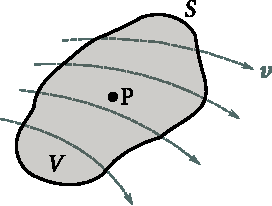
\includegraphics[scale=1]{figures/ch_01/fig_1_23.pdf}
		\caption[]{}
		\label{fig:1_23}
	\end{center}
	\vspace{-0.8cm}
\end{figure}

Thương số nhận được khi chia thông lượng $\Phi_v$ với thể tích,
\begin{equation}\label{eq:1_78}
	\frac{\Phi_v}{V}
\end{equation}

\noindent
cho công suất đơn vị trung bình của các nguồn giới hạn trong thể tích $V$. Giới hạn khi $V$ tiến tới không, tức là, thể tích $V$ co lại thành điểm P, biểu thức \eqref{eq:1_78} cho đúng công suất đơn vị của nguồn tại điểm P, gọi là \textbf{divergence} của vector $\vec{v}$ (được viết là $\diverg{\vec{v}}$). Do đó, theo định nghĩa,
\begin{equation*}
	\diverg{\vec{v}} = \lim_{V\to \text{P}} \frac{\Phi_v}{V}.
\end{equation*}

\noindent
Divergence của bất kì vector $\vec{a}$ được xác định theo cách tương tự:
\begin{equation}\label{eq:1_79}
	\diverg{\vec{a}} = \lim_{V\to \text{P}} \frac{\Phi_a}{V} = \lim_{V\to \text{P}} \frac{1}{V} \oint \vec{a} \ccdot \deriv{\vec{S}}.
\end{equation}

\noindent
Tích phân được lấy trên mặt kín $S$ tùy ý xung quanh điểm P\footnote{Vòng tròn trên dấu tích phân biểu thị rằng lấy tích phân trên một mặt kín.}; $V$ là thể tích giới hạn trong mặt này. Vì sự biến đổi $V\to$P được thực hiện khi $S$ tiến tới không, ta có thể giả sử rằng \eqn{1_79} không phụ thuộc vào hình dạng bề mặt. Giả định này được xác nhận bằng các tính toán chặt chẽ.

Ta hãy bao quanh điểm P bằng một mặt cầu có bán kính rất nhỏ $r$ (\fig{1_24}). Do $r$ rất nhỏ, thể tích $V$ bao quanh bởi hình cầu cũng sẽ rất nhỏ. Do đó với độ chính xác cao, ta có thể xem giá trị của $\diverg{\vec{a}}$ trong giới hạn của thể tích $V$ là không đổi\footnote{Giả sử rằng giá trị của $\diverg{\vec{a}}$ thay đổi liên tục, không có bước nhảy nào, khi đi từ một điểm của trường tới điểm khác.}. Trong trường hợp này, ta có thể viết phù hợp với \eqn{1_79} 
\begin{equation*}
	\Phi_a \approx (\diverg{\vec{a}}) V
\end{equation*}

\noindent
Với $\Phi_a$ là thông lượng của vector a qua bề mặt bao bọc thể tích $V$. Theo \eqn{1_77}, $\Phi_a$ bằng $\ab{N}{beg}$, số đường a bắt đầu bên trong $V$ nếu $\diverg{\vec{a}}$ tại điểm P dương, hoặc $\ab{N}{term}$, số đường a kết thúc bên trong $V$ nếu $\diverg{\vec{a}}$ tại điểm P âm.

Như trên thì các đường của vector $\vec{a}$ bắt đầu ở vùng lân cận gần một điểm nhất thì có divergence dương. Đường sức trường ``phân kỳ'' từ điểm này; ``nguồn'' của trường (\fig{1_24}a). Trái lại, trong vùng lân cận của một điểm có divergence âm, các đường của vector $\vec{a}$ kết thúc. Các đường sức trường ``hội tụ'' về điểm này; ``phần chìm'' của trường (\fig{1_24}b). Giá trị tuyệt đối của $\diverg{\vec{a}}$ càng lớn, số đường bắt đầu hoặc kết thúc ở vùng lân cận của điểm đã cho càng lớn.

Từ định nghĩa \eqref{eq:1_79} có thể thấy rằng divergence là một hàm vô hướng của tọa độ xác định vị trí các điểm trong không gian (ngắn gọn là---một hàm điểm). Định nghĩa \eqref{eq:1_79} là định nghĩa chung nhất độc lập với loại hệ tọa độ sử dụng.

\begin{figure}[!htb]
	\begin{minipage}[t]{0.5\linewidth}
		\begin{center}
			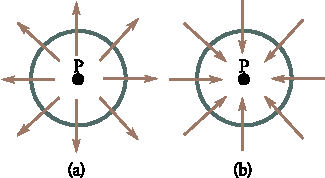
\includegraphics[scale=1.0]{figures/ch_01/fig_1_24.pdf}
			\caption[]{}
			\label{fig:1_24}
		\end{center}
	\end{minipage}
	\hspace{-0.05cm}
	\begin{minipage}[t]{0.5\linewidth}
		\begin{center}
			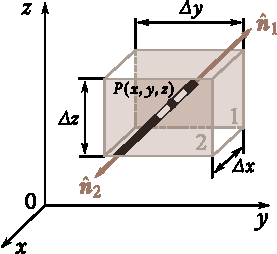
\includegraphics[scale=1.0]{figures/ch_01/fig_1_25.pdf}
			\caption[]{}
			\label{fig:1_25}
		\end{center}
	\end{minipage}
\vspace{-0.4cm}
\end{figure}

Ta hãy tìm biểu thức cho divergence trong hệ tọa độ Descartes. Xét một thể tích nhỏ dạng hình hộp với các cạnh song song với các trục tọa độ trong vùng lân cận điểm $P(x, y, z)$ (\fig{1_25}). Thông lượng vector qua mặt hình hộp được tính từ thông lượng qua từng mặt trong sáu mặt riêng lẻ.

Ta tìm thông lượng qua cặp mặt phẳng vuông góc trục $x$ (trong \fig{1_25} các mặt này được biểu diễn bằng các diện tích bóng mờ và đánh số 1 và 2). Ngoại hướng pháp tuyến $\hatvec{n}_2$ của mặt 2 trùng với hướng của trục $x$. Do đó, với các điểm trên mặt này, $a_{n_2}=a_x$. Ngoại hướng pháp tuyến $\hatvec{n}_1$ của mặt 1 ngược hướng với trục $x$. Do đó, với các điểm trên mặt này, $a_{n_1}=-a_x$. Thông lượng qua mặt 2 có thể được viết ở dạng
\begin{equation*}
	a_{x,2}\Delta{y}\Delta{z}
\end{equation*}

\noindent
với $a_{x,2}$ là giá trị trung bình của $a_x$ trên mặt 2. Thông lượng qua mặt 1 là
\begin{equation*}
	- a_{x,1}\Delta{y}\Delta{z}
\end{equation*}

\noindent
với $a_{x,1}$ là giá trị trung bình của $a_x$ trên mặt 1. Tổng thông lượng qua mặt 1 và 2 là
\begin{equation}\label{eq:1_80}
	(a_{x,2} - a_{x,1}) \Delta{y}\Delta{z}.
\end{equation}

Hiệu $a_{x,2}-a_{x,1}$ là độ tăng giá trị trung bình của $a_x$ khi dịch chuyển dọc theo trục $x$ khoảng $\Delta{x}$. Nhờ độ nhỏ của hình hộp (nhắc lại rằng ta sẽ cho kích thước của nó co lại về không), độ tăng này có thể viết ở dạng $(\diffinpartial{a_x}{x})\Delta{x}$, với giá trị $\diffinpartial{a_x}{x}$ lấy tại điểm P\footnote{Sự thiếu chính xác ta chấp nhận ở đây biến mất khi thể tích co lại thành điểm P trong biến đổi giới hạn.}. Do đó, \eqn{1_80} trở thành
\begin{equation*}
	\diffpartial{a_x}{x}\Delta{x}\Delta{y}\Delta{z} = \diffpartial{a_x}{x}\Delta{V}.
\end{equation*}

\noindent
Lập luận tương tự cho phép ta thu được các biểu thức sau cho thông lượng qua các cặp mặt vuông góc với trục $y$ và $z$:
\begin{equation*}
	\diffpartial{a_y}{y}\Delta{x}\Delta{y}\Delta{z} = \diffpartial{a_y}{y}\Delta{V},\quad \diffpartial{a_z}{z}\Delta{x}\Delta{y}\Delta{z} = \diffpartial{a_z}{z}\Delta{V}.
\end{equation*}

Do đó, thông lượng tổng cộng qua toàn bộ bề mặt kín được xác định bởi biểu thức
\begin{equation*}
	\Phi_a = \parenthesis{\diffpartial{a_x}{x} + \diffpartial{a_y}{y} + \diffpartial{a_z}{z}}\Delta{V}.
\end{equation*}

\noindent
Chia biểu thức này với $\Delta{V}$, ta sẽ tìm được divergence của vector a tại điểm $P(x, y, z)$:
\begin{equation}\label{eq:1_81}
	\diverg{\vec{a}} = \diffpartial{a_x}{x} + \diffpartial{a_y}{y} + \diffpartial{a_z}{z}.
\end{equation}

\textbf{Định lý Ostrogradsky-Gauss.} Nếu ta biết divergence của vector $\vec{a}$ tại mọi điểm trong không gian, ta có thể tính thông lượng của vector này qua mọi mặt kín có kích thước hữu hạn. Ta hãy làm điều này đầu tiên cho thông lượng vector $\vec{v}$ (thông lượng chất lỏng). Tích $\diverg{\vec{v}}$ và $\deriv{V}$ cho công suất của nguồn chất lỏng giới hạn trong thể tích $\deriv{V}$. Tổng của tích này $\int(\diverg{\vec{v}})\,\deriv{V}$, cho ta tổng công suất đại số của các nguồn giới hạn trong thể tích $V$ mà tích phân được lấy. Do chất lỏng không nén, tổng công suất của các nguồn phải bằng thông lượng chất lỏng chảy ra mặt $S$ bao quanh thể tích $V$. Vì thế ta có phương trình
\begin{equation*}
	\oint_S \vec{v} \ccdot \deriv{\vec{S}} = \int_V (\diverg{\vec{v}})\,\deriv{V}.
\end{equation*}

\noindent
Phương trình tương tự cho trường vector có bản chất bất kỳ:
\begin{equation}\label{eq:1_82}
	\oint_S \vec{a} \ccdot \deriv{\vec{S}} = \int_V (\diverg{\vec{a}})\,\deriv{V}.
\end{equation}

\noindent
Liên hệ này được gọi là định lý \textbf{Ostrogradsky-Gauss}. Tích phân bên trái được tính trên một mặt kín tùy ý $S$, và tích phân bên phải được tính trên thể tích $V$ bao bọc bởi bề mặt này.

\textbf{Lưu số.} Ta hãy trở lại với dòng chất lỏng lý tưởng không nén. Tưởng tượng một đường kín---chu tuyến $\Gamma$. Giả sử bằng một cách nào đó ta đóng băng ngay lập tức chất lỏng trong toàn bộ thể tích ngoại trừ một kênh kín rất mỏng có tiết diện không đổi bao gồm đường cong kín $\Gamma$ (\fig{1_26}). Tùy thuộc vào bản chất của trường vector vận tốc, chất lỏng trong kênh sẽ đứng yên hoặc chuyển động dọc đường cong kín (lưu thông) theo một trong hai hướng khả dĩ. Ta hãy lấy đại lượng bằng tích của vận tốc chất lỏng trong kênh và chiều dài đường cong kín $l$ như một cách đo lường chuyển động này. Đại lượng này được gọi là \textbf{lưu số} của vector $\vec{v}$ trên đường cong kín $\Gamma$. Do đó,
\begin{equation*}
	\text{lưu số của $\vec{v}$ trên $\Gamma$} = vl
\end{equation*}

\noindent
(Vì ta giả sử kênh có tiết diện không đổi, nên độ lớn của vận tốc, $v$, không đổi).

\begin{figure}[!htb]
	\begin{center}
		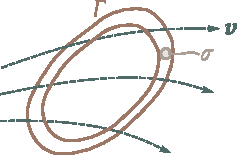
\includegraphics[scale=1]{figures/ch_01/fig_1_26.pdf}
		\caption[]{}
		\label{fig:1_26}
	\end{center}
	\vspace{-0.8cm}
\end{figure}

Tại thời điểm các bức tường đóng băng, thành phần vận tốc vuông góc với tường sẽ bị loại bỏ trong mỗi hạt chất lỏng, và chỉ còn lại thành phần vận tốc tiếp tuyến với đường cong kín $v_l$. Động lượng $\deriv{\vec{p}_l}$, gắn với thành phần này. Độ lớn của động lượng phần chất lỏng chứa trong một đoạn của kênh có chiều dài $\deriv{l}$ là $\rho\sigma v_l\,\deriv{l}$ ($\rho$ là khối lượng riêng chất lỏng, và $\sigma$ là tiết diện của kênh). Vì chất lỏng lý tưởng, tác động của các tường chỉ có thể đổi hướng vector $\deriv{\vec{p}_l}$, chứ không thay đổi độ lớn của nó. Sự sương tác giữa các hạt chất lỏng sẽ dẫn đến sự phân bố lại động lượng giữa chúng và làm cân bằng vận tốc của tất cả các hạt. Tổng đại số thành phần tiếp tuyến của động lượng không đổi: Động lượng một hạt tương tác nhận được bằng với động lượng bị mất của hạt thứ hai. Điều này chỉ ra rằng
\begin{equation*}
	\rho\sigma vl = \oint_{\Gamma} \rho \sigma v_l\,\deriv{l}
\end{equation*}

\noindent
với $v$ là vận tốc ổn định, và $v_l$ là thành phần tiếp tuyến của vận tốc chất lỏng trong thể tích $\sigma\,\deriv{l}$ tại thời điểm trước khi đóng băng. Rút gọn $\rho\sigma$, ta có
\begin{equation*}
	\text{lưu số của $\vec{v}$ trên $\Gamma$} = vl = \oint_{\Gamma} v_l\,\deriv{l}.
\end{equation*}

\noindent
Lưu số của bất kì vector $\vec{a}$ trên một đường kín tùy ý $\Gamma$ được xác định theo cách tương tự:
\begin{equation}\label{eq:1_83}
	\text{lưu số của $\vec{a}$ trên $\Gamma$} = \oint_{\Gamma} \vec{a} \ccdot \deriv{\vec{l}} = \oint_{\Gamma} a_l\,\deriv{l}.
\end{equation}

Có vẻ như khi lưu số khác không, các đường vector phải kín hoặc ít nhất bị uống cong theo cách nào đó hoặc khác theo hướng phá vỡ đường cong kín. Dễ thấy rằng giả thiết này sai. Ta hãy xét dòng chảy tầng của nước trong một con sông. Vận tốc của nước tại đáy sông bằng không và tăng dần khi ta tiếp cận mặt nước (\fig{1_27}). Đường dòng (đường vector $\vec{v}$) là đường thẳng. Mặc dù điều này, lưu số vector $\vec{v}$ trên đường cong kín minh họa bởi đường nét đứt hiển nhiên khác không. Mặt khác, trong trường có các đường cong,lưu số có thể bằng không.

\begin{figure}[!htb]
	\begin{minipage}[t]{0.5\linewidth}
		\begin{center}
			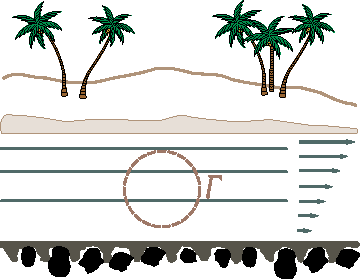
\includegraphics[scale=0.95]{figures/ch_01/fig_1_27.pdf}
			\caption[]{}
			\label{fig:1_27}
		\end{center}
	\end{minipage}
	\hspace{-0.05cm}
	\begin{minipage}[t]{0.5\linewidth}
		\begin{center}
			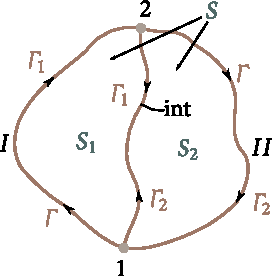
\includegraphics[scale=0.95]{figures/ch_01/fig_1_28.pdf}
			\caption[]{}
			\label{fig:1_28}
		\end{center}
	\end{minipage}
\vspace{-0.65cm}
\end{figure}

Lưu số có tính cộng. Điều này nghĩa là tổng lưu số trên đoạn $\Gamma_1$ và $\Gamma_2$ bao quanh bề mặt $S_1$ và $S_2$ (\fig{1_28}) bằng với thông lượng trên đoạn $\Gamma$ bao quanh bề mặt $S$, cái mà là ghép của bề mặt $S_1$ và $S_2$. Thật vậy, lưu số $C_1$ trên đoạn bao quanh bề mặt $S_1$ có thể biểu diễn như là tổng của các tích phân
\begin{equation}\label{eq:1_84}
	C_1 = \oint_{\Gamma_1} \vec{a} \ccdot \deriv{\vec{l}} = \int_{1,(I)}^2 \vec{a} \ccdot \deriv{\vec{l}} + \int_{2,(\text{int.})}^1 \vec{a} \ccdot \deriv{\vec{l}}.
\end{equation}

\noindent
Tích phân đầu tiên được lấy trên phần $I$ của đường bao ngoài, cái thứ hai lấy trên giao tuyến giữa mặt $S_1$ và $S_2$ theo hướng $2$-$1$.

Tương tự, lưu số $C_2$ lấy trên đoạn bao quanh bề mặt $S_2$ là
\begin{equation}\label{eq:1_85}
	C_2 = \oint_{\Gamma_2} \vec{a} \ccdot \deriv{\vec{l}} = \int_{2,(II)}^1 \vec{a} \ccdot \deriv{\vec{l}} + \int_{1,(\text{int.})}^2 \vec{a} \ccdot \deriv{\vec{l}}.
\end{equation}

\noindent
Tích phân đầu tiên được lấy trên phần $II$ của đường bao ngoài, cái thứ hai lấy trên giao tuyến giữa mặt $S_1$ và $S_2$ theo hướng $1$-$2$.

Lưu số trên đoạn giới hạn bề mặt $S$ có thể biểu diễn ở dạng
\begin{equation}\label{eq:1_86}
	C = \oint_{\Gamma} \vec{a} \ccdot \deriv{\vec{l}} = \int_{1,(I)}^2 \vec{a} \ccdot \deriv{\vec{l}} + \int_{2,(II)}^1 \vec{a} \ccdot \deriv{\vec{l}}.
\end{equation}

\noindent
Số hạng thứ hai trong phương trình \eqref{eq:1_84} và \eqref{eq:1_85} chỉ khác dấu nhau. Do đó, tổng các biểu thức này bằng \eqn{1_86}. Từ đó,
\begin{equation}\label{eq:1_87}
	C = C_1 + C_2.
\end{equation}

Phương trình \eqref{eq:1_87} ta đã chứng minh không phụ thuộc vào hình dạng bề mặt và đúng cho mọi số lượng số hạng. Từ đó, nếu ta chia một bề mặt mở $S$ tùy ý thành một lượng lớn bề mặt nguyên tố $\Delta{S}$\footnote{Trong hình, các mặt nguyên tố được mô tả ở dạng hình chữ nhật. Thực ra, hình dạng của chúng có thể hoàn toàn tùy ý.} (\fig{1_29}), thì lưu số trên đoạn bao quanh $S$ có thể viết dưới dạng tổng lưu số nguyên tố $\Delta{C}$ trên đoạn bao quanh $\Delta{S}$:
\begin{equation}\label{eq:1_88}
	C = \sum_i \Delta{C}_i.
\end{equation}

\begin{figure}[!htb]
	\begin{center}
		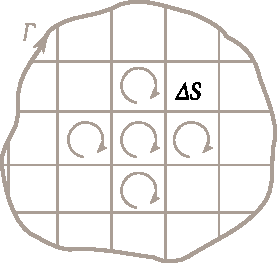
\includegraphics[scale=1]{figures/ch_01/fig_1_29.pdf}
		\caption[]{}
		\label{fig:1_29}
	\end{center}
	\vspace{-0.8cm}
\end{figure}

\textbf{Curl.} Tính cộng được của lưu số cho phép ta đưa ra khái niệm lưu số đơn vị, tức là, xét tỷ số giữa lưu số $C$ với độ lớn của bề mặt $S$ xung quanh nó lưu số ``chảy''. Với mặt $S$ hữu hạn, tỷ lệ $C/S$ cho giá trị trung bình của lưu số đơn vị. Giá trị này miêu tả đặc tính của trường trung bình trên mặt $S$. Để nhận được đặc trưng của trường tại điểm P, ta phải giảm kích thước bề mặt, làm nó co lại thành điểm P. Tỷ lệ $C/S$ tiến tới một giới hạn miêu tả đặc tính của trường tại điểm P.

Do đó, lấy một đường cong kín ảo $\Gamma$ trong một mặt phẳng đi qua điểm P, và xét biểu thức
\begin{equation}\label{eq:1_89}
	\lim_{S\to\text{P}} \frac{C_a}{S}
\end{equation}

\noindent
với $C_a$ là lưu số của vector $\vec{a}$ trên đoạn $\Gamma$ và $S$ là diện tích bề mặt giới hạn bởi đường cong kín.

Giới hạn \eqref{eq:1_89} được tính cho một mặt phẳng định hướng tùy ý không thể là một đặc tính toàn diện của trường tại P vì độ lớn của giới hạn này phụ thuộc vào hướng của đường cong kín trong không gian ngoài các đặc tính của trường tại điểm P. Hướng này có thể được cho bởi hướng của một pháp tuyến dương $\hatvec{n}$ đối với mặt phẳng đường cong kín (một pháp tuyến dương là cái mà liên kết với chiều di chuyển trên chu tuyến khi tích phân theo nguyên tắc nắm tay phải). Khi xác định giới hạn \eqref{eq:1_89} tại điểm P với hướng khác $\hatvec{n}$, ta sẽ nhận được giá trị khác. Với hướng ngược lại, giá trị này chỉ bị đổi dấu (sự đảo hướng $\hatvec{n}$ tương đương với sự đảo chiều di chuyển trên chu tuyến khi tích phân, cái mà chỉ làm đổi dấu lưu số ). Với một hướng xác định của pháp tuyến, độ lớn biểu thức \eqref{eq:1_89} tại điểm đã cho là cực đại.

Do đó, đại lượng \eqref{eq:1_89} như là hình chiếu của một vector lên hướng pháp tuyến của mặt phẳng chứa đường cong kín mà lưu số được lấy. Giá trị lớn nhất của đại lượng \eqref{eq:1_89} xác định độ lớn của vector này, và hướng của pháp tuyến dương $\hatvec{n}$ khi đạt giá trị lớn nhất là hướng của vector. Vector này gọi là \textbf{curl} của vector $\vec{a}$. Ký hiệu của nó là $\curl{\vec{a}}$. Sử dụng ký hiệu này, ta có thể viết biểu thức \eqref{eq:1_89} ở dạng
\begin{equation}\label{eq:1_90}
	(\curl{\vec{a}})_n = \lim_{S\to\text{P}} \frac{C_a}{S} = \lim_{S\to\text{P}} \frac{1}{S} \oint_S \vec{a}\, \deriv{\vec{l}}.
\end{equation}

Ta có thể nhận được hình ảnh minh họa về curl của vector $\vec{v}$ bằng cách tưởng tượng một cánh quạt nhỏ và nhẹ đặt tại điểm cho trước trong một chất lỏng đang chảy (\fig{1_30}). Tại những điểm mà curl khác không, cánh quạt sẽ quay, vận tốc nó càng lớn, khi giá trị hình chiếu của curl lên trục cánh quạt càng lớn.

Phương trình \eqref{eq:1_90} xác định vector $\curl{\vec{a}}$. Định nghĩa này là cái chung nhất mà không phụ thuộc vào loại hệ tọa độ sử dụng. Để tìm biểu thức cho hình chiếu của vector $\curl{\vec{a}}$ lên các trục tọa độ descartes, ta phải xác định giá trị của đại lượng \eqref{eq:1_90} theo hướng của diện tích $S$ mà pháp tuyến $\hatvec{n}$ của diện tích trùng với một trong các trục $x, y, z$. Giả sử, ta hướng $\hatvec{n}$ dọc theo trục $x$, từ đó \eqref{eq:1_90} trở thành $(\curl{\vec{a}})_x$.
Chu tuyến $\Gamma$ trong trường hợp này nằm trong mặt phẳng song song với mặt phẳng tọa độ $yz$. Ta lấy đường cong kín này ở dạng hình chữ nhật với cạnh $\Delta{y}$ và $\Delta{z}$ (\fig{1_31}, trục $x$ hướng về chúng ta trong hình này; chiều di chuyển biểu diễn trong hình liên kết với hướng của trục $x$ bởi định luật nắm tay phải). Đoạn $1$ của đường cong kín ngược hướng với trục $z$. Do đó, $a_l$ trên đoạn này là $-a_z$. Với lý do tương tự, $a$ trên đoạn $2$, $3$, và $4$ bằng $a_y$, $a_z$, và $-a_y$, tương ứng. Từ đó, lưu số có thể viết ở dạng
\begin{equation}\label{eq:1_91}
	\parenthesis{a_{z,3} - a_{z,1}} \Delta{z} - \parenthesis{a_{y,4} - a_{y,2}} \Delta{y}
\end{equation}

\noindent
Với $a_{z,3}$ và $a_{z,1}$ là giá trị trung bình của $a_z$ trên đoạn $3$ và $1$, tương ứng, $a_{y,4}$ và $a_{y,2}$ là giá trị trung bình của $a_{y}$ trên đoạn $4$ và $2$.

\begin{figure}[!htb]
	\begin{minipage}[t]{0.5\linewidth}
		\begin{center}
			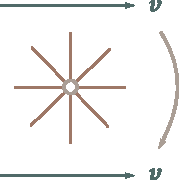
\includegraphics[scale=1]{figures/ch_01/fig_1_30.pdf}
			\caption[]{}
			\label{fig:1_30}
		\end{center}
	\end{minipage}
	\hspace{-0.1cm}
	\begin{minipage}[t]{0.5\linewidth}
		\begin{center}
			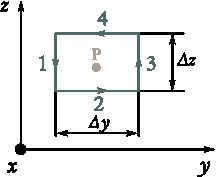
\includegraphics[scale=1]{figures/ch_01/fig_1_31.pdf}
			\caption[]{}
			\label{fig:1_31}
		\end{center}
	\end{minipage}
\vspace{-0.4cm}
\end{figure}

Hiệu $a_{z,3}-a_{z,1}$ là độ tăng giá trị trung bình của $a_z$ trên đoạn $\Delta{z}$ khi đoạn này dịch chuyển theo hướng của trục $y$ đoạn $\Delta{y}$. Nhờ độ nhỏ của $\Delta{y}$ và $\Delta{z}$, độ tăng này có thể biểu diễn ở dạng $(\diffinpartial{a_z}{y})\Delta{y}$, với giá trị của $\diffinpartial{a_z}{y}$ lấy tại điểm P\footnote{Sự thiếu chính xác ta chấp nhận ở đây biến mất khi đường bao co lại thành điểm P trong biến đổi giới hạn.}. Tương tự, hiệu $a_{y,4}-a_{y,2}$ có thể biểu diễn ở dạng $(\diffinpartial{a_y}{z})\Delta{z}$.
Sử dụng những biểu thức này trong \eqn{1_91} và đặt nhân tử chung ngoài dấu ngoặc đơn, ta nhận được biểu thức sau đây cho lưu số:
\begin{equation*}
	\parenthesis{\diffpartial{a_z}{y} - \diffpartial{a_y}{z}} \Delta{y}\Delta{z} = \parenthesis{\diffpartial{a_z}{y} - \diffpartial{a_y}{z}} \Delta{S}
\end{equation*}

\noindent
với $\Delta{S}$ là diện tích của đường cong kín. Chia lưu số cho $\Delta{S}$, ta được biểu thức cho hình chiếu của $\curl{\vec{a}}$ lên trục $x$:
\begin{equation}\label{eq:1_92}
	(\curl{\vec{a}})_x = \diffpartial{a_z}{y} - \diffpartial{a_y}{z}.
\end{equation}

\noindent
Bằng cách tương tự ta có thể tìm được
\begin{align}
	(\curl{\vec{a}})_y &= \diffpartial{a_x}{z} - \diffpartial{a_z}{x}, \label{eq:1_93}\\
	(\curl{\vec{a}})_z &= \diffpartial{a_y}{x} - \diffpartial{a_x}{y}. \label{eq:1_94}
\end{align}

Có thể dễ thấy rằng bất kỳ phương trình \eqref{eq:1_92}-\eqref{eq:1_94} có thể nhận được từ cái trước đó [\eqn{1_94} được xem như cái trước của \eqn{1_92}] bởi cái gọi là sự chuyển vị tuần hoàn của các tọa độ, tức là, thay thế các tọa độ theo cơ chế
\begin{equation*}
	\begin{tikzcd}[column sep=small]
x \arrow[rr, bend left] &           & y \arrow[ld, bend left] \\
                        & z \arrow[lu, bend left] &
\end{tikzcd}
\end{equation*}

Do đó, curl của vector $\vec{a}$ được xác định trong hệ tọa độ Descartes bởi biểu thức sau:
\begin{equation}\label{eq:1_95}
	\curl{\vec{a}} = \vecuni{x}\parenthesis{\diffpartial{a_z}{y} - \diffpartial{a_y}{z}} + \vecuni{y}\parenthesis{\diffpartial{a_x}{z} - \diffpartial{a_z}{x}} + \vecuni{z}\parenthesis{\diffpartial{a_y}{x} - \diffpartial{a_x}{y}}.
\end{equation}

\noindent
Dưới đây ta sẽ chỉ ra một cách tinh tế hơn để viết biểu thức này.

\textbf{Định lý Stokes.} Biết curl của vector $\vec{a}$ tại mọi điểm trên mặt $S$ (không nhất thiết là mặt phẳng), ta có thể tính lưu số của vector này trên chu tuyến $\Gamma$ giới hạn $S$ (chu tuyến cũng có thể không nằm trong một mặt phẳng). Vì ý định này, ta chia bề mặt thành các phần tử rất nhỏ $\Delta{S}$. Do độ nhỏ của chúng, những phần tử này có thể xem như mặt phẳng. Do đó theo \eqn{1_90}, lưu số của vector $\vec{a}$ trên đường cong kín giới hạn $\Delta{S}$ có thể viết ở dạng
\begin{equation}\label{eq:1_96}
	\Delta{C} \approx (\curl{\vec{a}})_n \Delta{S} = \curl{\vec{a}} \ccdot \Delta{\vec{S}}
\end{equation}

\noindent
Với $\hatvec{n}$ là một pháp tuyến dương của phần tử bề mặt $\Delta{S}$.

Theo \eqn{1_88}, tổng của biểu thức \eqref{eq:1_96} trên tất cả $\Delta{S}$ dẫn đến lưu số của vector $\vec{a}$ trên đường cong kín $\Gamma$ giới hạn $S$:
\begin{equation*}
	C = \sum\Delta{C} \approx \sum\curl{\vec{a}} \ccdot \Delta{\vec{S}}.
\end{equation*}

\noindent
Thực hiện biến đổi giới hạn tất cả $\Delta{S}$ tiến tới không (số lượng của chúng tăng không giới hạn), ta được phương trình
\begin{equation}\label{eq:1_97}
	\oint_{\Gamma} \vec{a}\ccdot\deriv{\vec{l}} = \int_S (\curl{\vec{a}}) \ccdot \Delta{\vec{S}}.
\end{equation}

\noindent
Phương trình \eqref{eq:1_97} gọi là \textbf{Định lý Stokes}. Ý nghĩa của nó là lưu số của vector $\vec{a}$ trên một đường cong kín tùy ý $\Gamma$ bằng thông lượng của vector $\curl{\vec{a}}$ qua bề mặt tùy ý $S$ giới hạn bởi đường cong kín cho trước.

\textbf{Toán tử Del}. Viết công thức phân tích vector được đơn giản hóa đáng kể nếu ta đưa vào một toán tử vi phân ký hiệu bởi biểu tượng $\nabla$ (nabla hoặc del) và gọi là \textbf{toán tử del} hoặc \textbf{toán tử Hamilton}. Toán tử này biểu diễn một vector với các thành phần $\diffinpartial{}{x}$, $\diffinpartial{}{y}$ và $\diffinpartial{}{z}$. Kết quả là,
\vspace{-10pt}
\begin{equation}\label{eq:1_98}
	\nabla = \vecuni{x}\diffpartial{}{x} + \vecuni{y}\diffpartial{}{y} + \vecuni{z}\diffpartial{}{z}.
\end{equation}

\noindent
Vector này tự nó không có nghĩa. Nó có nghĩa khi kết hợp với hàm vô hướng hoặc hàm vector mà nó được nhân một cách tượng trưng. Do đó, nếu ta nhân vector $\nabla$ với hàm vô hướng $\varphi$ ta được vector
\begin{equation}\label{eq:1_99}
	\gradop{\varphi} = \vecuni{x}\diffpartial{\varphi}{x} + \vecuni{y}\diffpartial{\varphi}{y} + \vecuni{z}\diffpartial{\varphi}{z}
\end{equation}

\noindent
Là gradient của hàm $\varphi$ [xem \eqn{1_68}].

Tích vô hướng của vector $\nabla$ và $\vec{a}$ cho ta hàm vô hướng
\begin{equation}\label{eq:1_100}
	\divop{\vec{a}} = \nabla_{x}a_{x} + \nabla_{y}a_{y} + \nabla_{z}a_{z}
\end{equation}

\noindent
mà ta có thể xem như divergence của vector $\vec{a}$ [xem \eqn{1_81}].

Cuối cùng, tích vector của vector $\nabla$ và $\vec{a}$ cho ta một vector với các thành phần $(\curlop{\vec{a}})_x=\nabla_{y}a_{z} - \nabla_{z}a_{y}=\diffinpartial{a_z}{y}-\diffinpartial{a_y}{z}$, vân vân., trùng với các thành phần của $\curl{\vec{a}}$ [xem Phương trình. \eqref{eq:1_92}-\eqref{eq:1_94}]. Từ đó, sử dụng cách viết tích vector bằng định thức, ta có
\begin{equation}\label{1_101}
	\curl{\vec{a}} = \curlop{\vec{a}} = \begin{vmatrix}
	\vecuni{x} & \vecuni{y} & \vecuni{z}\\
	\diffpartial{}{x} & \diffpartial{}{y} & \diffpartial{}{z}\\
	a_x & a_y & a_z
	\end{vmatrix}.
\end{equation}

Do đó, có hai cách biểu diễn gradient, divergence, và curl:
\begin{equation*}
	\gradop{\varphi}\equiv\grad{\varphi},\quad \divop{\vec{a}}\equiv\diverg{\vec{a}},\quad \curlop{\vec{a}}\equiv\curl{\vec{a}}.
\end{equation*}

\noindent
Việc sử dụng ký hiệu del có một số ưu điểm. Do đó ta sẽ sử dụng ký hiệu này trong phần sau. Người ta đã quen nhận định ký hiệu $\gradop{\varphi}$ là ``gradient của phi'' (tức là, không nói ``del phi'', mà là ``gradient of phi''), ký hiệu $\divop{\vec{a}}$ là ``divergence của a'' và, cuối cùng, ký hiệu $\curlop{\vec{a}}$ là ``curl của a''.

Khi sử dụng vector $\nabla$, phải nhớ rằng nó là toán tử vi phân tác dụng lên tất cả hàm ở bên phải của nó. kết quả là, trong các biểu thức biến đổi chứa $\nabla$, ta phải xem xét cả hai quy tắc của đại số vector và giải tích vi phân. Ví dụ, đạo hàm của tích hàm số $\varphi$ và $\psi$ là
\begin{equation*}
	(\varphi\psi)' = \varphi'\psi + \varphi\psi'.
\end{equation*}

\noindent
Do đó,
\begin{equation}\label{eq:1_102}
	\grad{(\varphi\psi)} = \gradop{(\varphi\psi)} = \psi\gradop{\varphi} + \varphi\gradop{\psi} = \psi\,\grad{\varphi} + \varphi\,\grad{\psi}.
\end{equation}

\noindent
Tương tự,
\begin{equation}\label{eq:1_103}
	\diverg{(\varphi\vec{a})} = \divop{(\varphi\vec{a})} = \vec{a}\ccdot(\gradop{\varphi}) + \varphi(\divop{\vec{a}}).
\end{equation}

Gradient của hàm $\varphi$ là một hàm vector. Do đó, divergence và curl có thể áp dụng lên nó:
\begin{align}
	\diverg{\grad{\varphi}} &= \divop{\gradop{\varphi}} = (\divop{\nabla})\varphi = \parenthesis{\nabla_x^2 + \nabla_y^2 + \nabla_z^2}\varphi\nonumber\\
	&= \diffsecpartial{\varphi}{x} + \diffsecpartial{\varphi}{y} + \diffsecpartial{\varphi}{z} = \upDelta{\varphi}\label{eq:1_104}
\end{align}

\noindent
($\upDelta$ là toán tử Laplace)
\begin{equation}\label{eq:1_105}
	\curl{\grad{\varphi}} = \curlop{(\gradop{\varphi})} = (\curlop{\nabla})\varphi
\end{equation}

\noindent
(nhớ rằng tích vector của một vector với chính nó là không).

Ta hãy áp dụng divergence và curl lên hàm $\curl{\vec{a}}$:
\begin{equation}\label{eq:1_106}
	\diverg{\curl{\vec{a}}} = \divop{\curlop{\vec{a}}} = 0
\end{equation}

\noindent
(một tích vô hướng bội ba bằng với thể tích của một hình hộp được xây dựng trên các vector được nhân (xem Tập I, phần 22); nếu có hai vector trong số đó trùng nhau, thể tích của hình hộp bằng không):
\begin{equation}\label{eq:1_107}
	\curl{\curl{\vec{a}}} = \curlop{(\curlop{\vec{a}})} = \gradop{(\divop{\vec{a}})} - (\divop{\nabla})\vec{a} = \grad{\diverg{\vec{a}}} - \upDelta{\vec{a}}
\end{equation}

\noindent
[ta đã sử dụng phương trình (1.35) của tập I, cụ thể là, $\vec{a}\times\vec{b}\times\vec{c} = \vec{b}(\vecdot{a}{c}) - \vec{c}(\vecdot{a}{b})$].

Phương trình \eqref{eq:1_106} chỉ ra rằng trường của curl không có nguồn. Từ đó, các đường sức của vector $\curl{\vec{a}}$ không có điểm bắt đầu cũng như kết thúc. Chính vì lý do này mà thông lượng của curl qua bất kì bề mặt $S$ tựa lên đường cong kín cho trước $\Gamma$ là như nhau [xem \eqn{1_97}).

Ta sẽ lưu ý ở kết luận khi toán tử del được sử dụng, Phương trình \eqref{eq:1_82} và \eqref{eq:1_97} có thể ở dạng
\begin{align}
	\oint_S \vec{a} \ccdot \deriv{\vec{S}} &= \oint_V \divop{\vec{a}}\, \deriv{V},\quad\quad\! \text{(Định lý Ostrogradsky-Gauss)}\label{eq:1_108}\\
	\oint_{\Gamma} \vec{a} \ccdot \deriv{\vec{l}} &= \int_S (\curlop{\vec{a}}) \ccdot \deriv{\vec{S}}.\quad \text{(Định lý Stokes)}\label{eq:1_109}
\end{align}

\section{Lưu Số và Curl của Trường Tĩnh Điện}\label{sec:1_12}

Chúng ta đã thành lập ở \sect{1_6} rằng lực tác dụng lên điện tích $q$ trong trường tĩnh điện có tính bảo toàn. Vì thế, công mà lực này thực hiện trên một đường cong kín $\Gamma$ bằng không:
\begin{equation*}
	A = \oint_{\Gamma} q\vec{E} \ccdot \deriv{\vec{l}} = 0.
\end{equation*}

\noindent
Triệt tiêu $q$, chúng ta có
\begin{equation}\label{eq:1_110}
	\oint_{\Gamma} \vec{E} \ccdot \deriv{\vec{l}} = 0
\end{equation}

\noindent
(so sánh với \eqn{1_46}]

Tích phân ở vế trái của \eqn{1_110} là lưu số vector điện trường $\vec{E}$ trên toàn chu tuyến $\Gamma$ [xem phép khai triển \eqref{eq:1_80}]. Do đó, \textit{một trường tĩnh điện luôn có lưu số vector điện trường của một đường cong kín bất kì bằng không}.

Chọn một mặt $S$ nằm trên chu tuyến $\Gamma$, với lưu số điện trường đã biết (\fig{1_32}). Theo định lý Stokes [xem \eqn{1_109}], tích phân của $\curl{\vec{E}}$ trên toàn bộ bề mặt bằng với lưu số vector điện trường $\vec{E}$ trên toàn chu tuyến $\Gamma$:
\begin{equation}\label{eq:1_111}
	\int_S (\curlop{\vec{E}}) \ccdot \deriv{\vec{S}} = \oint_{\Gamma} \vec{E} \ccdot \deriv{\vec{l}}.
\end{equation}

\noindent
Mặt khác lưu số bằng không, nên ta sẽ có
\begin{equation*}
	\int_S (\curlop{\vec{E}}) \ccdot \deriv{\vec{S}} = 0.
\end{equation*}

\noindent
Điều kiện này là luôn đúng với mọi mặt $S$ nằm trên chu tuyến $\Gamma$ bất kì. Miễn là curl của vector $\vec{E}$ tại một điểm bất kì trong không gian bằng không:

\begin{equation}\label{eq:1_112}
	\curlop{\vec{E}} = 0.
\end{equation}

\begin{figure}[!htb]
	\begin{minipage}[t]{0.5\linewidth}
		\begin{center}
			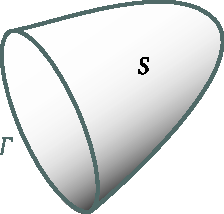
\includegraphics[scale=0.95]{figures/ch_01/fig_1_32.pdf}
			\caption[]{}
			\label{fig:1_32}
		\end{center}
	\end{minipage}
	\hspace{-0.1cm}
	\begin{minipage}[t]{0.5\linewidth}
		\begin{center}
			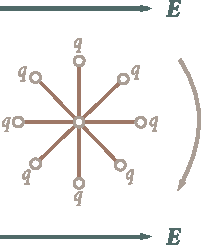
\includegraphics[scale=0.95]{figures/ch_01/fig_1_33.pdf}
			\caption[]{}
			\label{fig:1_33}
		\end{center}
	\end{minipage}
\vspace{-0.4cm}
\end{figure}

Ta xét mô hình quạt ở \fig{1_25}, với mỗi đầu của nó được đính những điện tích dương $q$ (\fig{1_33}; toàn bộ hệ này phải có kích thước rất nhỏ). Nếu tại một điểm bất kì trong điện trường mà $\curl{\vec{E}}$ khác không, mô hình ta đề cập ở trên sẽ quay với một gia tốc tỉ lệ thuận với hình chiếu của curl lên trục quay. Nhưng, với trường tĩnh điện, những mô hình như trên sẽ không quay theo bất kì hướng nào.

Như thế, đặc điểm của trường tĩnh điện là nó không phải là trường xoáy. Chúng ta đã chứng tỏ được điều này vì curl của gradient của một hàm vô hướng luôn bằng không [xem biến đổi ở \eqref{eq:1_96}]. Vì thế, việc $\curl{\vec{E}}$ bằng không tại mọi điểm trong không gian giúp ta viết được biểu thức của $\vec{E}$ dưới dạng gradient của hàm vô hướng (mà ta đã biết nó là điện thế). Chúng ta đã xem xét biểu thức này ở \sect{1_8} [xem \eqn{1_41}; dấu trừ của biểu thức này được suy ra từ các lập luận vật lý]. 

Theo điều kiện từ \eqref{eq:1_110}, thì ta sẽ lập tức nhận ra rằng trường tĩnh điện ở \fig{1_34} là bất khả thi. Với một trường như hình trên, thì lưu số quanh một chu tuyến, mô tả bởi đường nét đứt, thì khác không. Điều này sẽ mâu thuẫn với điều kiện \eqref{eq:1_110}. Nó cũng bất khả thi với việc tồn tại một điện trường đều (khác không) bên trong một thể tích xác định (\fig{1_35}). Trong trường hợp này chu tuyến mô tả bởi đường nét đứt sẽ có lưu số khác không.

\begin{figure}[!htb]
	\begin{minipage}[t]{0.36\linewidth}
		\begin{center}
			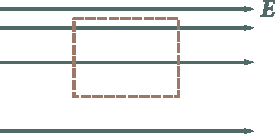
\includegraphics[scale=0.93]{figures/ch_01/fig_1_34.pdf}
			\caption[]{}
			\label{fig:1_34}
		\end{center}
	\end{minipage}
	% \hspace{-0.05cm}
	\hfill{ }
	\begin{minipage}[t]{0.2\linewidth}
		\begin{center}
			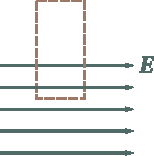
\includegraphics[scale=0.93]{figures/ch_01/fig_1_35.pdf}
			\caption[]{}
			\label{fig:1_35}
		\end{center}
	\end{minipage}
	% \hspace{-0.05cm}
	\hfill{ }
	\begin{minipage}[t]{0.37\linewidth}
		\begin{center}
			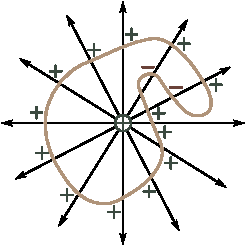
\includegraphics[scale=0.95]{figures/ch_01/fig_1_36.pdf}
			\caption[]{}
			\label{fig:1_36}
		\end{center}
	\end{minipage}
\vspace{-0.45cm}
\end{figure}

\section{Định Luật Gauss}\label{sec:1_13}

Chúng ta đã tính được curl trong một trường tĩnh điện ở chương trước. Giờ chúng ta sẽ đi tìm divergence của nó. Để bắt đầu, chúng ta thử xét trường của một điện tích điểm $q$ và tính thông lượng vector $\vec{E}$ qua diện tích mặt kín $S$ bao lấy điện tích (\fig{1_36}). Chúng ta đã biết được từ \sect{1_5} rằng tổng số đường sức vector $\vec{E}$ phân kỳ từ $q$ hay hội tụ tại $-q$ đều có giá trị đại số là $q/\varepsilon_0$.

Từ \eqn{1_77} ta biết rằng thông lượng của vector $\vec{E}$ qua một diện tích mặt kín bằng với số đường sức thoát ra (nếu điện tích dương), hoặc số đường sức đâm vào (nếu điện tích âm). Cho rằng số đường sức thoát ra hay đâm vào đều có giá trị đại số bằng $q/\varepsilon_0$ (xem \sect{1_5}), chúng ta có thể viết được
\begin{equation}\label{eq:1_113}
	\Phi_E = \frac{q}{\varepsilon_0}.
\end{equation}

\noindent
Dấu của thông lượng phụ thuộc vào dấu của $q$. Thứ nguyên của hai vế là giống nhau.

Giờ chúng ta xét một mặt kín chứa $N$ điện tích $q_1, q_2, \ldots, q_N$. Theo nguyên lý chồng chất, cường độ $\vec{E}$ của hệ sẽ là tổng hợp các cường độ $\vec{E_i}$ của từng điện tích: $\vec{E}=\sum_i\vec{E}_i$
\begin{equation*}
	\Phi_E = \oint_S \vec{E}\ccdot\deriv{\vec{S}} = \oint_S \parenthesis{\sum_i\vec{E}_i}\ccdot\deriv{\vec{S}} = \sum_i\oint_S\vec{E}_i\ccdot\deriv{\vec{S}}.
\end{equation*}

\noindent
Mỗi tích phân bên trong dấu sum bằng $q_i/\varepsilon_0$. Vì thế,
\begin{equation}\label{eq:1_114}
	\Phi_E = \oint_S \vec{E}\ccdot\deriv{\vec{S}} = \frac{1}{\varepsilon_0} \sum_{i=1}^N q_i.
\end{equation}

\noindent
Biểu thức chúng ta vừa tìm được được gọi là \textbf{định luật Gauss}. Dựa theo định lý, \textit{thông lượng của vector điện trường qua diện tích mặt kín bằng với tổng đại số điện tích được chứa trong mặt kín chia cho $\varepsilon_0$}.

Khi xem xét trường tạo ra bởi một hệ điện tích vĩ mô (là hệ được cấu tạo từ vô số các điện tích nguyên tố), ta bỏ qua sự rời rạc trong cấu trúc, và cho rằng nó được phân bố trong không gian liên tục với một mật độ xác định tại mọi nơi. \textbf{Mật độ điện tích khối của một điện tích} $\rho$ được xác định tương tự với khối lượng riêng. Chỉ khác là, ta lấy tỉ lệ giữa $\deriv{q}$ trên một thể tích nhỏ vô hạn (theo quan điểm vật lý) $\deriv{V}$ mà chứa điện tích trên:
\begin{equation}\label{eq:1_115}
	\rho = \diff{q}{V}.
\end{equation}

\noindent
Khi nói về một thể tích rất nhỏ, chúng ta phải hiểu rằng đó là thể tích chứa một lượng điện tích xác định và phân bố đều trong thể tích ấy. Tuy nhiên, vùng thể tích này phải rất lớn so với thể tích của một điện tích nguyên tố riêng lẻ.

Biết được mật độ điện khối trong không gian, chúng ta có thể tính được tổng điện tích được giữ bên trong bề mặt kín $S$. Để tính được điện tích, ta cần phải lấy tích phân của $\rho$ trên toàn bộ thể tích bị giới hạn bởi mặt kín $S$.
\begin{equation*}
	\sum_i q_i = \int_V \rho\,\deriv{V}.
\end{equation*}

\noindent
Ngoài ra, \eqn{1_114} có thể được viết là
\begin{equation}\label{eq:1_116}
	\oint_S \vec{E}\ccdot\deriv{\vec{S}} = \frac{1}{\varepsilon_0} \int_V \rho\,\deriv{V}.
\end{equation}

Theo tích phân Gauss (\eqn{1_108}), chúng ta sẽ có
\begin{equation*}
	\int_V \divop{\vec{E}}\,\deriv{V} = \frac{1}{\varepsilon_0} \int_V \rho\,\deriv{V}.
\end{equation*}

\noindent
Phương trình mà chúng ta vừa thành lập có thể sử dụng cho mọi miền thể tích $V$. Điều này có nghĩa là các biểu thức bên trong dấu tích phân phải bằng nhau tại mọi điểm trong không gian. Từ đây, ta thấy rằng liên hệ giữa divergence của vector $\vec{E}$ và mật độ điện khối là

\begin{equation}\label{eq:1_117}
	\divop{\vec{E}} = \frac{1}{\varepsilon_0} \rho.
\end{equation}

\noindent
Phương trình này còn được gọi là dạng vi phân của định lý Gauss.

Khi xét một dòng chảy chất lỏng, $\divop{\vec{v}}$ cho biết công suất được thực hiện bởi nguồn tại một điểm xác định. Tương tự, đối với tĩnh điện thì điện tích được coi tương tự như nguồn nước ở trường hợp trên. 

\section{Một Số Vận Dụng Của Định Luật Gauss }\label{sec:1_14}

Định luật Gauss cho phép chúng ta tính toán cường độ điện trường một cách đơn giản hơn việc sử dụng $\eqn{1_15}$ để tổng hợp cường độ điện trường của từng điện tích điểm. Một số ví dụ sau đây sẽ có thể cho ta thấy được sự tiện lợi của định luật Gauss. Điều này sẽ giúp chúng ta rất nhiều trong nghiên cứu sâu hơn về điện trường. Trước khi bắt đầu, chúng ta nên tiếp cận đến khái niệm mật độ điện mặt và mật độ điện dài.

Nếu một vật có điện tích được phân bố đều trên bề mặt của nó, thì sự phân bố đó sẽ được đặc trưng bằng đại lượng $\sigma$, hay còn được biết đến là mật độ điện mặt, được xác định bằng
\begin{equation}\label{eq:1_118}
	\sigma = \diff{q}{S}.
\end{equation}

\noindent
Ở đây $\deriv{q}$ là điện tích nằm trong phần diện tích $\deriv{S}$. Với $\deriv{S}$ là diện tích vi phân.

Nếu điện tích được phân bố dọc theo độ dài của một ống trụ (Xét mặt cắt vuông góc với trục ống, mật độ điện mặt của nó là không đổi trên toàn mặt đó), chúng ta sẽ sử dụng đại lương gọi là \textit{mật độ điện dài}
\begin{equation}\label{eq:1_119}
	\lambda = \diff{q}{l}
\end{equation}

\noindent
Ở đây, $\deriv{l}$ là độ dài vi phân dọc theo độ dài dây, và $\deriv{q}$ là điện tích chứa trong ống trụ vi phân trên.

\textbf{Điện trường của Mặt Phẳng Vô Hạn phân bố đều.} Ta giả sử rằng mật độ điện mặt tại mọi điểm là xác định và đều bằng $\sigma$; để tổng quát hoá biểu thức, ta cho rằng điện tích là dương. Do tính đối xứng của sự vô hạn, điện trường sẽ có hướng vuông góc với mặt phẳng. Bởi vì, do tấm rộng vô hạn và phân bố điện tích đều, nên không lý do gì để vector $\vec{E}$ bị nghiêng so với phương vuông góc mặt phẳng. Hai miền đối diện nhau được chia cắt bởi bờ là mặt phẳng vô hạn, cường độ điện trường của chúng cùng độ lớn và ngược chiều nhau.

\begin{figure}[!htb]
	\begin{minipage}[t]{0.5\linewidth}
		\begin{center}
			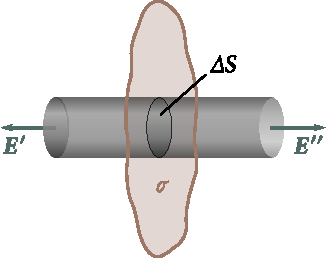
\includegraphics[scale=1]{figures/ch_01/fig_1_37.pdf}
			\caption[]{}
			\label{fig:1_37}
		\end{center}
	\end{minipage}
	\hspace{-0.05cm}
	\begin{minipage}[t]{0.5\linewidth}
		\begin{center}
			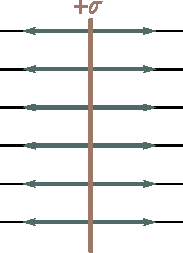
\includegraphics[scale=1]{figures/ch_01/fig_1_38.pdf}
			\caption[]{}
			\label{fig:1_38}
		\end{center}
	\end{minipage}
\vspace{-0.4cm}
\end{figure}

Giờ chúng ta giả sử có một ống trụ, trục của nó vuông góc với mặt phẳng, đáy có diện tích bằng $\Delta{S}$, ống trụ đối xứng hai bên (trung điểm thuộc bề mặt tích điện). Bởi vì đối xứng, chúng ta có $E'=E''=E$. Ta áp dụng định luật Gauss cho các mặt này. Thông lượng qua diện tích mặt bên của ống trụ bằng không, vì $E_n$\footnote{$E_n$ là vector điện trường vuông góc với bề mặt đang xét} tại mỗi điểm đều vuông góc với mặt trụ bên. Tại ngay trên bề mặt, $E_n$ trùng với $E$. Tổng thông lượng qua mặt là $2E\Delta{S}$. Điện tích của mặt phẳng được chứa trong mặt trụ là $\sigma\Delta{S}$. Theo định luật Gauss, ta sẽ có
\begin{equation*}
	2E\Delta{S} = \frac{\sigma\Delta{S}}{\varepsilon_0}
\end{equation*}

\noindent
suy ra
\begin{equation}\label{eq:1_120}
	E = \frac{\sigma}{2\varepsilon_0}.
\end{equation}

\noindent
Kết quả mà chúng ta nhận được không phụ thuộc vào chiều dài của ống trụ mà ta xét. Điều này cho ta thấy rằng cường độ điện trường có độ lớn không phụ thuộc vào khoảng cách đến mặt. Đường sức được mô tả ở \fig{1_38}. Nếu với trường hợp điện tích âm, kết quả vẫn như vậy, chỉ khác là vector $\vec{E}$ và đường sức bị đảo chiều.

Nếu mặt phẳng mà chúng ta xét không phải vô hạn, ví dụ như một đĩa mỏng bị tích điện\footnote{Đối với một đĩa, $\sigma$ ở \eqn{1_120} nên được hiểu là điện tích chứa trong \SI{1}{\metre\squared} nhân độ dày của nó. Với vật dẫn kim loại, điện tích được phân bố trên mặt ngoài của nó. Nên nếu ta xét một mặt của nó thì ta có $\sigma$ chỉ bằng một nửa khi xét toàn đĩa.}, thì kết quả trên chỉ còn đúng cho những điểm mà khoảng cách của nó tới rìa mặt phẳng rất lớn so với khoảng cách của nó đến bề mặt tích điện (trong \fig{1_39} vùng dưới đường nét đứt là vùng chúng ta đang nói tới). Khi xét một điểm càng xa bản tụ hoặc đến gần rìa của nó, thì nó không còn được coi là mặt phẳng vô hạn nữa. Dễ thấy rằng, khi đặt mặt phẳng vào một không gian rộng, thì điện trường mà nó gây ra giống như một điện tích điểm.

\textbf{Điện Trường của Hai Mặt Phẳng Tích Điện Đều.} Điện trường gây ra bởi hai mặt phẳng rộng vô hạn với độ lớn mật độ điện mặt không đổi $\sigma$ có thể tính được dựa vào tổng hợp điện trường của từng mặt (\fig{1_40}). Ở khoảng không gian giữa hai mặt phẳng, điện trường được tổng hợp cùng hướng, nên nó có giá trị là
\begin{equation}\label{eq:1_121}
	E = \frac{\sigma}{\varepsilon_0}.
\end{equation}

\noindent
Ở vùng không gian bên ngoài hai mặt phẳng thì điện trường triệt tiêu nhau nên nó có giá trị bằng không tại mọi điểm.

\begin{figure}[!htb]
	\begin{minipage}[t]{0.5\linewidth}
		\begin{center}
			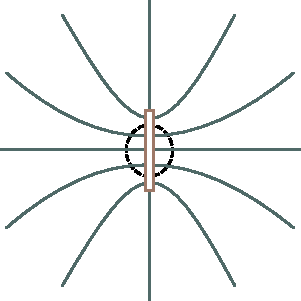
\includegraphics[scale=1]{figures/ch_01/fig_1_39.pdf}
			\caption[]{}
			\label{fig:1_39}
		\end{center}
	\end{minipage}
	\hspace{-0.05cm}
	\begin{minipage}[t]{0.5\linewidth}
		\begin{center}
			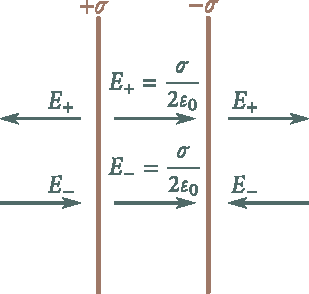
\includegraphics[scale=1]{figures/ch_01/fig_1_40.pdf}
			\caption[]{}
			\label{fig:1_40}
		\end{center}
	\end{minipage}
\vspace{-0.55cm}
\end{figure}

Vì thế, điện trường chỉ tồn tại ở giữa hai mặt phẳng tích điện. Điện trường này có giá trị không đổi và chỉ hướng về một phía; vì thế, nó là điện trường đều. Đường sức điện là những đường thẳng song song cách đều nhau.

Kết quả mà chúng ta nhận được cũng đúng cho trường hợp mặt phẳng không vô hạn, nhưng khoảng cách giữa chúng là vô cùng bé so với độ rộng của chúng (nó còn được gọi là tụ điện phẳng). Trong trường hợp này, tại rìa của chúng, có xuất hiện những sai lệch so với các tính toán trên của ta (như \fig{1_41}).

\textbf{Điện Trường của Mặt Trụ Tích Điện.} Cho rằng ống trụ (bán kính R) có mật độ điện mặt không đổi là $\sigma$. Vì tính đối xứng, nên điện trường gây ra bởi ống trụ có phương xuyên tâm, và giá trị của nó chỉ phụ thuộc vào khoảng cách $r$ đến trục ống trụ. Chúng ta vẽ ra một mặt trụ đồng trục có bán kính $r$ và độ cao là $h$. Với mặt đáy của hình trụ, chúng ta có $E_n=0$ (Ta giả sử điện tích là dương). Vì thế ta có thế tính điện thông của vector $\vec{E}$ qua mặt này bằng $E(r)\times 2\pi rh$. Nếu $r>R$, điện tích là $q=\lambda h$ (với $\lambda$ là mật độ điện dài) được chứa trong mặt trụ. Áp dụng định lý Gauss, ta có thể tìm được 
\begin{equation*}
	E(r)\times 2\pi rh = \frac{2\lambda}{\varepsilon_0}.
\end{equation*}

\noindent
Do đó,
\begin{equation}\label{eq:1_122}
	E(r) = \frac{1}{2\pi\varepsilon_0}\frac{\lambda}{r}\quad (r\geqslant R).
\end{equation}

\noindent
Nếu $r<R$, không có điện tích nào được chứa bên trong mặt trụ, vì thế $E(r)=0$.

\begin{figure}[!htb]
	\begin{minipage}[t]{0.35\linewidth}
		\begin{center}
			
\includegraphics[scale=1]{figures/ch_01/fig_1_41.pdf}
			\caption[]{}
			\label{fig:1_41}
		\end{center}
	\end{minipage}
	\hspace{-0.05cm}
	\begin{minipage}[t]{0.65\linewidth}
		\begin{center}
			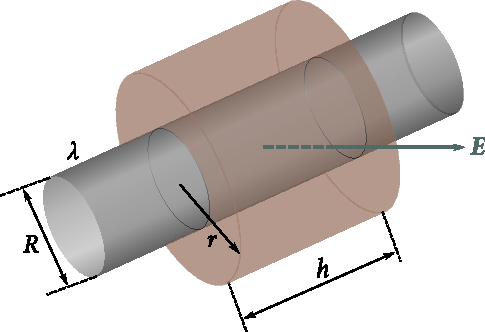
\includegraphics[scale=0.95]{figures/ch_01/fig_1_42.pdf}
			\caption[]{}
			\label{fig:1_42}
		\end{center}
	\end{minipage}
\vspace{-0.4cm}
\end{figure}

Cũng từ đó ta thấy được rằng, nó không tồn tại điện trường bên trong một ống trụ tích điện đều dài vô hạn. Điện trường ở không gian bên ngoài thì phụ thuộc vào mật độ điện tích dài $\lambda$ và khoảng cách tới trục $r$.

Đối với ống trụ tích điện âm, thì chỉ khác ở chiều của điện trường $\vec{E}$ bên ngoài ống. Theo \eqn{1_112}, khi ta càng tiến gần về phía bề mặt của ống trụ (với mật độ $\lambda$ không đổi), thì điện trường có giá trị càng lớn. Và nó đạt giá trị lớn nhất tại ngay mặt của ống trụ. 

Ta có $\lambda=2\pi R\sigma$, thế nó vào $\eqn{1_122}$ và xét tại $r=R$, chúng ta sẽ nhận được điện trường tại gần bề mặt trụ là: 
\begin{equation}\label{eq:1_123}
	E(R) = \frac{\sigma}{\varepsilon_0}.
\end{equation}

Chúng ta có thể tính được điện trường do hai ống trụ đồng trục (tích mật độ như nhau nhưng trái dấu) tạo ra bằng nguyên lý chồng chất ($\fig{1_43}$). Ta nhận thấy rằng, không có điện trường bên trong ống trụ nhỏ hay bên ngoài ống trụ lớn. Điện trường ở vùng không gian giữa hai mặt được xác định thông qua $\eqn{1_122}$. Điều này cũng đúng cho ống trụ hữu hạn nhưng khoảng cách giữa hai mặt là rất bé (được gọi là tụ trụ). Khi lại gần rìa của ống trụ, thì điện trường tại đó sẽ bị sai lệch so với những tính toán ta đã làm trên.

\begin{figure}[!htb]
	\begin{center}
		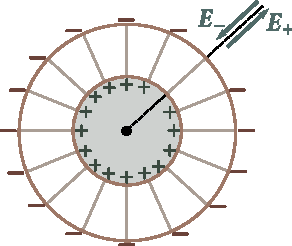
\includegraphics[scale=1]{figures/ch_01/fig_1_43.pdf}
		\caption[]{}
		\label{fig:1_43}
	\end{center}
	\vspace{-0.8cm}
\end{figure}

\textbf{Điện trường của Mặt Cầu Tích Điện.} Điện trường tạo ra bởi một mặt cầu có bán kính $R$ được tích điện với mật độ đều $\sigma$ là đối xứng qua tâm. Điều này có nghĩa là phương của vector $\vec{E}$ sẽ đi qua tâm của hình cầu, với độ lớn của $\vec{E}$ là một hàm của $r$ tính từ tâm. Ta dựng một măt cầu đồng tâm với quả cầu trên. Với mọi điểm trên bề mặt này, thì $E_n=E(r)$. Nếu $r>R$, thì toàn bộ điện tích trên quả cầu đều nằm trong mặt cầu. Vì thế,
\begin{equation*}
	E(r)\times 4\pi r^2 = \frac{q}{\varepsilon_0}
\end{equation*}

\noindent
whence hay
\begin{equation}\label{eq:1_124}
	E(r) = \frac{1}{4\pi\varepsilon_0}\frac{q}{r^2}.\quad (r\geqslant R)
\end{equation}

Với mặt cầu có bán kính $r$ bé hơn $R$ nó sẽ không chứa điện tích, vì thế với $r<R$ thì chúng ta có $E(r)=0$.

Do đó, không có điện trường ở bên trong quả cầu tích điện với mật độ mặt đều $\sigma$. Bên ngoài quả cầu, điện trường sẽ tương tự như một điện tích điểm, có giá trị bằng tổng điện tích của quả cầu và đặt tại tâm.

Theo nguyên lý chồng chất điện trường, chúng ta có thể dễ dàng tính điện trường giữa hai mặt cầu đồng tâm (còn được gọi là tụ cầu) mang lần lượt điện tích $+q$ và $-q$ có cùng giá trị xác định. Điện trường có thể được tính thông qua \eqn{1_124}.

\textbf{Điện Trường của Quả Cầu Điện Tích.} Cho một quả cầu bán kính $R$ có điện tích phân bố đều bên trong quả cầu với một mật độ $\rho$. Điện trường trong trường hợp là đối xứng xuyên tâm. Ta dễ dàng thấy rằng, điện trường bên ngoài của nó giống như ở trường hợp mặt cầu tích điện ta xét vừa rồi [xem \eqn{1_124}]. Nhưng kết quả sẽ khác nhau khi xét bên trong lòng quả cầu. Lấy một mặt cầu bán kính $r$ (với $r<R$), điện trường chứa bên trong nó là $\rho\times 4\pi r^3/3$. Thế nên, định luật Gauss cho mặt này ta được:
\begin{equation*}
	E(r)\times 4\pi r^2 = \frac{1}{\varepsilon_0}\rho \frac{4}{3}\pi r^3.
\end{equation*}

\noindent
Ta thay $q/(4\pi R^3/3)$ bằng $\rho$, ta sẽ có
\begin{equation}\label{eq:1_125}
	E(r) = \frac{1}{4\pi\varepsilon_0}\frac{q}{R^3}r.\quad (r\leqslant R)
\end{equation}

Từ đấy, ta thấy rằng điện trường bên trong quả cầu có dạng tuyến tính phụ thuộc theo $r$ (tính từ tâm). Bên ngoài quả cầu, điện trường tương tự với một điện tích đặt ở tâm quả cầu.
